\documentclass[12pt,openany]{book}
\usepackage[T1]{fontenc}
\usepackage[english]{babel}
\usepackage[babel=true]{csquotes}
\usepackage{parskip}
\usepackage{placeins}
\usepackage{import}
\usepackage{helvet}
\usepackage{geometry}
\usepackage{enumitem}
\usepackage{booktabs}
\usepackage[labelfont=bf]{caption}
\usepackage{mathtools}
\usepackage{amsmath}
\usepackage{esint}
\usepackage{extarrows}
\usepackage{amssymb}
\usepackage{amsthm}
\usepackage[mleftright]{diffcoeff}
\usepackage{tikz-cd}
\usepackage{tikz}
\usepackage{natbib}
\usepackage[hidelinks]{hyperref}
\usepackage[english]{cleveref}
\usepackage{tocloft}
\usepackage{enumitem}
\setlist[enumerate]{label=(\roman*)}

\usepackage{MA_Titlepage}

% % Fix spacing before TOC title and between title and entriesem}
\setlength{\cftbeforetoctitleskip}{-3em}  % space before "Contents"
\setlength{\cftaftertoctitleskip}{2em}  % space after "Contents" and before entries

% Indent chapter entries
\setlength{\cftchapindent}{0pt}
\setlength{\cftsecindent}{1.5em}  % or however much you want

% === page settings ============================================================
\pagestyle{headings}
\geometry{scale=.666, marginratio=1:1, heightrounded}
%================================================
\newtheoremstyle{plainnormal}  % Name of the style
  {\topsep}                    % Space above
  {\topsep}                    % Space below
  {\normalfont}               % Body font (upright)
  {}                          % Indent amount
  {\bfseries}                 % Theorem head font (bold)
  {.}                         % Punctuation after theorem head
  { }                         % Space after theorem head
  {}                          % Theorem head spec
\newcommand{\R}{\mathbb{R}}
\def\S{\mathcal{S}}
\theoremstyle{plainnormal}
% "Theorem" environments (bold header, italic body)
\newtheorem{theorem}{Theorem}[section]
\newtheorem{lemma}[theorem]{Lemma}
\newtheorem{definition}[theorem]{Definition}
\newtheorem{remark}[theorem]{Remark}
\newtheorem{algorithm}[theorem]{Algorithm}
\newenvironment{abstract}{
  \cleardoublepage
  \null\vfill
  \begin{center}\bfseries Abstract\end{center}
  \begin{quote}
}{
  \end{quote}
  \vfill\null
  \cleardoublepage
}
% "Remark" environments (italic header, upright body)
\theoremstyle{remark}
\newtheorem*{note}{Note}
% define reference name for "\cref{...}"
\crefname{notation}{Notation}{Notations}
% === math settings ============================================================
% equations are numbered with preceding section
\counterwithin{equation}{section}
% operators

\DeclareMathOperator*{\argmin}{arg\,min}

\AddToHook{cmd/section/before}{\clearpage}

\makeatletter
\renewcommand*{\fps@figure}{htbp}
\renewcommand*{\fps@table}{htbp}

\AddToHook{cmd/@floatboxreset/after}{\centering}
\AddToHook{cmd/@floatboxreset/after}{\centering}
\makeatother
%Name of the author of the thesis 
\authornew{Johann Samuel Weidemaier}
%Date of birth of the Author
\geburtsdatum{10th July 2001}
%Place of Birth
\geburtsort{Heidelberg, Germany}
%Date of submission of the thesis
\date{\today}
%Name of the Advisor
% z.B.: Prof. Dr. Peter Koepke
\betreuer{Advisor: Prof. Dr. Martin Rumpf}
%name of the second advisor of the thesis
\zweitgutachter{Second Advisor: Prof. Dr. Sergio Conti}

\institut{Institut f\"ur Numerische Simulation}
%Title of the thesis 
\title{A framework for \\ neural geometric PDEs\\on neural implicit surfaces}
%Do not change!
\ausarbeitungstyp{Master's Thesis  Mathematics}
\date{\today}
\begin{document}
\pagestyle{empty}
\pagenumbering{roman}

\maketitle

\pagestyle{headings}
\setcounter{page}{5}

\begingroup
\let\clearpage\relax

\begin{abstract}
This thesis presents a neural framework for solving geometric partial differential equations (PDEs) on neural implicit manifolds. We first introduce a novel approach for constructing highly accurate signed distance functions (SDFs) from unoriented point clouds by replacing the commonly used Eikonal equation with a neural variational heat-based approach. Similar approaches have been used in the past to compute distances on discrete surfaces, but these have yet to be applied in a neural setting. Our approach consists of two convex optimization problems: First, we compute a neural approximation of the heat equation using a small time step and a density-dependent approximation of the surface measure as initial data. Secondly, we use the normalized gradients of the heat solution to compute the SDF. Utilizing this approach, we construct two different SDF methods, one focusing on global and one on local approximation. We show that the underlying variational problems are well-posed for both methods.
Through numerical experiments, we demonstrate that our methods provide state-of-the-art surface reconstruction and consistent SDF gradients.\par
Finally, we present a novel neural framework for solving geometric PDEs. We address this by adapting the well-known narrow-band method from the discrete to the neural setting. Discrete narrow-band methods have shown to be exceptionally powerful when working with complex geometries; an adaptation using neural networks will allow to examine the new field of neural geometric PDEs. Providing various examples, we demonstrate that combining the heat-based neural SDF method with the neural narrow-band approach can accurately solve PDEs on the zero-level set.
\end{abstract}
\section*{Acknowledgments}
\endgroup
First and foremost, I would like to express my sincere gratitude to my supervisor, Prof. Martin Rumpf, for his continuous support, valuable guidance, and insightful discussions throughout the course of this thesis.
\par
I would also like to thank Florine Hartwig, Dr. Josua Sassen, Prof. Sergio Conti, Prof. Mirela Ben-Chen, and Prof. Martin Rumpf, with whom parts of this work were developed in collaboration. This collaboration led to the publication of the paper:\\
\hspace{0.5em}\\
\textit{Samuel Weidemaier, Florine Hartwig, et al., "SDFs from Unoriented Point Clouds using Neural Variational
Heat Distances", 2025.}\\
\hspace{0.5em}
\\
The work leading to this publication was supported by the Deutsche Forschungsgemeinschaft (DFG, German Research Foundation) via project 211504053 -- Collaborative Research Center 1060 and via Germany’s Excellence Strategy project 390685813 -- Hausdorff Center for Mathematics.
Furthermore, this project has received funding from the European Union’s Horizon 2020 research and innovation program under the Marie Skłodowska-Curie grant agreement No. 101034255, as well as the Israel Science Foundation (grant No. 1073/21).\\
Some of the ideas and results presented in this thesis are based on this joint work.\par 
\noindent
Finally, I am deeply grateful to my family and my girlfriend for their constant support and encouragement throughout my studies, particularly during the preparation of this thesis.
\clearpage

\tableofcontents

\section{Introduction}
\begin{figure}
    \centering
    \includegraphics[width=0.85\linewidth]{Figures/teaser_beethoven2.pdf}
    \caption{We present a framework that is capable of learning high-quality signed distance functions from unoriented point clouds (\textbf{top left}). These neural SDFs not only provide accurate representations of the zero-level set geometry (\textbf{top right}) but are also sufficiently smooth and provide reliable gradients to enable the numerical solution of partial differential equations using narrow-band methods. As a demonstration, we show that our approach can be used to compute a time step of the heat equation (\textbf{bottom right}) and subsequently approximate geodesic distances via a neural variant of the heat method (\textbf{bottom left}). }
    \label{teaser}
\end{figure}
This thesis proposes a novel approach to numerically approximate signed distance functions (SDFs) from unoriented point clouds using neural networks. In a second step, we utilize these neural SDFs to solve geometric partial differential equations (PDEs) using a neural narrow-band approach.\par
After revisiting the basic concepts from the calculus of variations, differential geometry, and neural networks (\Cref{ch:prelim}), we turn our attention to the computation of SDFs using a variational heat-based ansatz (\Cref{SectionNeuralImplicitSurf}). To this end, we replace the commonly used Eikonal equation ($\|\nabla \phi\| = 1$) with the heat method, thus carrying over to a neural setting what has long been standard practice for computing distances on discrete surfaces. This approach requires first the neural approximation of the unsigned gradients through a small time step of the heat equation. Using a second neural network, we then orient the gradient directions and fix the zero-level set to approximate the SDF. Using the methods from \cref{ch:prelim}, we show that both minimization problems are well-posed. This approach is based on ideas developed in joint work published in \cite{weidemaier2025sdfsunorientedpointclouds}. Furthermore, we present novel ideas on how to adapt and improve this method. Through numerical experiments, we demonstrate that our method provides state-of-the-art surface reconstruction and consistent SDF gradients.\par
The second part of the thesis presents, to our knowledge, a new framework for neural geometric PDEs, a class of PDEs in which the solution is governed by intrinsic geometric properties of the domain (\Cref{NPDEsonSurfaces}); for this, we extend the classical narrow-band method, used for example in combination with geometric finite elements and difference methods, to a neural setting. In various examples, we demonstrate that our SDF approach in combination with the neural narrow-band method is accurate enough to solve PDEs on the zero-level set.\par
Further technical details related to the proofs in \cref{SectionNeuralImplicitSurf}, as well as additional experiments, are provided in the Appendix (\Cref{appendix:A,appendix:B}).
\newpage
\pagenumbering{arabic}
\chapter{Preliminaries}\label{ch:prelim}
In this chapter, we recall the fundamental mathematical concepts that form the basis of the methods developed later in this thesis. Our goal is to approximate signed distance functions from unoriented point clouds using a variational ansatz and subsequently solve geometric partial differential equations using neural networks, both based on rigorous mathematical theory. For this purpose, we begin by revisiting the core ideas of the following areas:
\begin{itemize}
    \item \emph{Calculus of variations}, with a focus on the formulation and analysis of variational problems and their connection to partial differential equations.
    
    \item \emph{Variational neural networks}, which integrate neural function approximation into variational principles, allowing the neural solution of PDEs.
    
    \item Elements of \emph{differential geometry}, which are essential for formulating and analyzing PDEs on implicit manifolds.
\end{itemize}
These keystones will equip the reader with the necessary mathematical background to follow the subsequent developments and analysis.\par
For most of the theorems in this section, we will omit the proofs and refer the reader to standard textbooks, cited at the beginning of the respective section.
\section{Variational Calculus and Neural Networks}
We begin with an introduction to the basic concept of the calculus of variations; thereafter, we will discuss its application in the context of neural networks. For a complete introduction to the calculus of variations, see, for example, \cite{Dacorogna}. For a detailed overview of mathematical neural networks, we refer to \cite{e2020mathematicalunderstandingneuralnetworkbased}.
\begin{definition}
Let X be a real Banach space with norm $\|\cdot\|_X$, and let $I: X\rightarrow\R$ be a map.
\begin{itemize}
    \item \textbf{Lower semicontinuity:} $I$ is called (weakly) \emph{lower semicontinuous} if for each (weakly) convergent sequence $(u_n)_n$ with (weak) limit u, it holds
\[\liminf_{n \to \infty} I (u_n) \geq I(u)\]
    \item \textbf{Coercivity:} $I$ is called \emph{coercive} if for all $\|u_n\|_X\xrightarrow{n\rightarrow\infty} \infty:$ $ I(u_n) \rightarrow \infty$.
    \item \textbf{Weierstrass theorem:} Assume that $X$ is reflexive and $I$ is bounded below, coercive and weakly lower semicontinuous. Then I admits a minimizer, i.e., it exists $u_0 \in X \text{ s.t. } I(u_0) \leq I(u)$ for all $ u \in X$.
    \label{Weierstrass}
\end{itemize}
    
\end{definition}
\begin{lemma}\label{thm:Tonelli}\textbf{(Tonelli:)}
    Let $\Omega \in \R^n$ and $F:\R^m\rightarrow\R^{\pm\infty}$ be continuous. Then the integral functional $$u \mapsto \int_\Omega F(u(x))\,\mathrm{d}x$$
    is weakly lower semicontinuous in $L^p$ ,$1<p<\infty$, if and only if $F$ is convex.
\end{lemma}
\begin{definition}\textbf{(Quasiconvexity and Polyconvexity:)}
Let $f:\mathbb{R}^{m\times n} \to \mathbb{R}$ be a Borel function (i.e. the preimage of every open set is a Borel set).  
\begin{itemize}
    \item \textbf{Quasiconvexity:} Let $f$ be locally integrable (integrable over every compact subset). $f$ is called \emph{quasiconvex} if for every $A \in \mathbb{R}^{m\times n}$, bounded open $\Omega \subset \mathbb{R}^n$, and $\varphi \in W^{1,\infty}_0(\Omega;\mathbb{R}^m)$,
\[
f(A) \leq \frac{1}{|\Omega|} \int_{\Omega} f\bigl(A + \nabla\varphi(x)\bigr)\,\mathrm{d}x .
\]
\item \textbf{Polyconvexity:} $f$ is called \emph{polyconvex} if there exists a convex function $g$ on the space of all minors of matrices in $\mathbb{R}^{m\times n}$ such that $f(A) = g(\mathcal{M}(A))$, where $\mathcal{M}(A)$ is the vector of all minors of $A$.  
\item Every \emph{polyconvex} function is \emph{quasiconvex}.
\end{itemize}

\end{definition}

\begin{theorem}\label{thm:quasiconv}\textbf{(Quasiconvexity and weak lower semicontinuity):}
Let $\Omega\subset\mathbb{R}^n$ be a bounded open set and let
\(
f:\mathbb{R}^{m\times n}\to\mathbb{R}
\) be continuous. Assume that there is a constant $C\geq0$ and $1\leq p < \infty$ such that for all $A\in\mathbb{R}^{m\times n}$
\[
-C(1+|A|^q) \le f(A) \le C\bigl(1+|A|^p\bigr), \quad 1\leq q < p.
\]
If the map $A\mapsto f(A)$ is quasiconvex, then the integral functional
\[
I(u):=\int_\Omega f\bigl(\nabla u(x)\bigr)\,\mathrm{d}x
\]
is weakly lower semicontinuous on $W^{1,p}(\Omega;\mathbb{R}^m)$.
\end{theorem}

\begin{definition}\textbf{(Gateaux differentiability:)}
    Let $X$ be a real Banach space and let \mbox{$I: X\rightarrow\R$} be a map. Then $I$ is called \emph{Gateaux differentiable} at $u\in X$, if for all $w\in X$ the map $$\R \rightarrow\R, \quad \tau \mapsto I(u + \tau w)$$ is differentiable at $\tau = 0$.
\end{definition}
\begin{definition}\label{EL_eq}\textbf{(Euler-Lagrange equation:)}
Let X be a real Banach space and let \mbox{$I: X\rightarrow\R$} be a map. Assume $u_0\in X$ is a minimizer of $I$ on $X$ and $I$ is Gateaux differentiable at $u_0$. Then the minimizer $u_0$ is a solution of the \emph{Euler-Lagrange equation} $$I'(u_0)(w) = 0, \quad \text{for all } w \in X.$$
\end{definition}

\begin{definition}\textbf{(Artificial neural network:)}
   Let \( L \in \mathbb{N} \) denote the number of layers, and let \( (n_0, n_1, \dots, n_L) \in \mathbb{N}^{L+1} \) be the dimensions of each layer, where \( n_0 \) is the input dimension and \( n_L \) is the output dimension. An \textit{artificial neural network} is a function $\mathcal{N}_\theta$, where $\theta$ denotes its trainable parameters:
\[
\mathcal{N}_\theta: \mathbb{R}^{n_0} \rightarrow \mathbb{R}^{n_L},
\]
defined by the recursive composition of affine transformations and nonlinear activation functions. Specifically, for input \( x \in \mathbb{R}^{n_0} \), the output is computed recursively as
\[
x^{(0)} \coloneqq x, \quad x^{(l)} \coloneqq \sigma^{(l)}(W^{(l)} x^{(l-1)} + b^{(l)}) \quad \text{for } l = 1, \dots, L,
\]
where for each \( l \in \{1, \dots, L\} \):
\begin{itemize}
    \item \( W^{(l)} \in \mathbb{R}^{n_l \times n_{l-1}} \) is the weight matrix,
    \item \( b^{(l)} \in \mathbb{R}^{n_l} \) is called bias vector,
    \item \( \sigma^{(l)}: \mathbb{R}^{n_l} \rightarrow \mathbb{R}^{n_l} \) is an activation function.
\end{itemize}
A widely used activation function is \emph{ReLU}, $\sigma_{\text{ReLU}}(x) \coloneqq \max(0, x),$
due to its cheap computation and straightforward application within mathematical proofs. Other widely used activation functions are \emph{Sigmoid}, $\sigma(x) \coloneqq \frac{1}{1+e^{-x}} $, and \emph{hyperbolic tangent}, $\sigma(x) \coloneqq\tanh(x)$.
In this work, we will exclusively use the sinusoidal activation function \emph{SIREN} (\cite{sitzmann2020implicitneuralrepresentationsperiodic}): $$\sigma_{\text{SIREN}}(x) \coloneqq \sin(\omega_0 x),$$
which is applied component-wise in $x_i$.
\end{definition}
Neural networks are capable of approximating functions based on both empirical data and mathematical formulations, with the latter being essential for solving PDEs. In particular, \cite{HORNIK1989359} demonstrated that multilayer feedforward neural networks with nonlinear and bounded activation functions are universal approximators; thus, they can approximate any Borel-measurable function on a compact subset of $\R^n$ to arbitrary accuracy, given a sufficient number of hidden units. This \emph{universal approximation theorem} has been generalized over the past years; especially, boundedness is not a requirement, implying that, for example, ReLU activated networks are universal approximators, see \cite{petersen2018optimalapproximationpiecewisesmooth}. \par
Now that we have introduced the notion of a neural network, let us elaborate on the two main methods that have been proposed to solve PDEs using networks; for a detailed overview, we refer to \cite{E_2021}. First, the \emph{deep Ritz method} (\cite{deepritzmethoddeep}) uses the connection of minimization problems and PDEs, approximating the PDE by minimizing its variational form. As an example, in case of the Poisson problem, \begin{equation}\label{eq:triangle_strongform}
-\Delta u = f \text{ on } \Omega, \quad u = g \text{ on } \partial \Omega,
\tag{$\triangle$}
\end{equation} where $\Omega \subset \R^n $ is bounded, one typically minimizes the functional \begin{equation}\label{eq:star_weakform}
    I(u) \coloneqq \int_\Omega \frac{1}{2} \|\nabla u\|^2 - fu \,\mathrm{d}x + \lambda\int_{\partial \Omega} (u(x)- g(x))^2\, \mathrm{da},\tag{$\star$}
\end{equation}
where $u(x) = \mathcal N_\theta(x)$ for some set of trainable parameters $\theta$, and fixed $\lambda\in \R^+$. Then one seeks to approximate a minimizer, typically using stochastic gradient descent. Note that here and in the following, $\|\cdot\|$ denotes the vector norm in $\R^3$ and $\R^+$ are the positive real numbers. Minimizers of \cref{eq:star_weakform} are weak solutions of \cref{eq:triangle_strongform}, which can be seen by considering the Euler-Lagrange equation. We prefer this approach over other neural PDE methods, since the existence of minimizers of functionals similar to $I(u)$ can often be shown using the methods of variational calculus.\par
The more convenient alternative to the Deep Ritz method is often referred to as a \emph{Physics Informed Neural Network} (PINN), see \cite{RAISSI2019686}. PINNs minimize the squared residual of the respective PDE, for example, in the case of Poisson's equation the functional
$$  I_{PINN}(u) \coloneqq \int_\Omega |\Delta u + f|^2 \,\mathrm{d}x\, +\, \lambda \int_{\partial\Omega}(u(a) - g(a))^2 \, \mathrm{da}  .$$
Both the Deep Ritz method and PINNs demonstrate comparable approximation quality in practice and no significant empirical advantage has been consistently observed for a variety of problems for one method over the other, \cite{yang2025numericalstudyhyperparameter}. 
Here we want to point out that the PINN framework requires the computation of higher-order derivatives, which leads to increased computational effort. Furthermore, the PINN approach is, in general, numerically more unstable.
\section{Differential Geometry}
Within this section, we define the notion of a signed distance function in $\R^3$ and elaborate its key properties. Afterwards, we will recall the definitions of differential operators on implicit surfaces. Note that most of the following results generalize naturally to $\R^n$. However, since the focus of this thesis will be surfaces embedded in $\R^3$, we restrict the following theoretical framework to the case $n=3$.\par
For a more general introduction to differential geometry, see, for example, \cite{Lee00}, or, more specifically for implicit manifolds, \cite{Dziuk_Elliott_2013}. Regarding the theory on geodesics, we refer to \cite{Dacorogna}.
\begin{definition}\textbf{(Manifolds and embedded surfaces:)}
A \emph{smooth manifold} \(\mathcal{M}\) of dimension \(n\) is a topological space such that for every point \(p \in \mathcal{M}\), there exists an open neighborhood \(U \subseteq \mathcal{M}\) and a homeomorphism (i.e., a continuous bijection with continuous inverse) 
\(
\varphi: U \to V,
\)
onto an open subset \(V \subseteq \mathbb{R}^n\). Moreover, the \emph{transition maps} 
\(
\varphi_j \circ \varphi_i^{-1} : \varphi_i(U_i \cap U_j) \to \varphi_j(U_i \cap U_j)
\)
between overlapping charts shall be smooth functions between open subsets of \(\mathbb{R}^n\).
\par
A \emph{smooth embedded submanifold} \(\mathcal{M} \subset \mathbb{R}^n\) of dimension \(k\) is a subset, such that for every point \(x \in \mathcal{M}\), there exists an open neighborhood \(U \subset \mathbb{R}^n\) and a smooth embedding \(f: \mathbb{R}^k \to \mathbb{R}^n\) with \(f(\mathbb{R}^k) \cap U = \mathcal{M} \cap U\).\par
In particular, a \emph{smooth surface} \(\mathcal{S} \subset \mathbb{R}^3\) is a 2-dimensional embedded submanifold of \(\mathbb{R}^3\).
\end{definition}

\begin{definition}\label{defInsOuts}\textbf{(Inside/Outside of a surface:)}
    Let $\S$ be a smooth surface in $\R^3$. Let $\S$ further be compact, connected, orientable (i.e., admitting a continuous choice of unit normal vectors), and closed. Then we call the unbounded component of $\R^3\setminus \S$ the \emph{outside} of $\S$; further we call the bounded component of $\R^3\setminus \S$ the \emph{inside} of $\S$.
\end{definition}
\begin{remark}
    Note for completeness, that the existence of exactly two connected components, one bounded and one unbounded, is given by the \emph{Jordan-Brouwer Separation Theorem}. For a proof, see, for example, \cite{Lima01011988}. 
\end{remark}
\begin{definition}\textbf{(Signed distance function:)}
    Let $\S$ be a smooth surface that admits the assumptions of \cref{defInsOuts}. A \emph{signed distance function} (SDF) associated to $\S$ is a scalar function 
    $$\phi: \R^3 \rightarrow \R$$
    such that:
    $$\phi(x) = 
\begin{cases}
\phantom{-}\mathrm{d}(x, \S) & \text{if } x \text{ is outside } \S \\
\phantom{-} 0 & \text{if } x \in \S \\
-\mathrm{d}(x, \S) & \text{if } x \text{ is inside } \S
\end{cases} $$
    where $\mathrm{d} (x, \S)= \inf_{y\in \S} \|x - y\|$ is the Euclidean distance.
\end{definition}
    \begin{remark}
        While it would be more general to define
    $$|\phi(x)| = 
\begin{cases}
\mathrm{d}(x, \S) & \text{if } x \notin \S \\
0 & \text{if } x \in \S \\
\end{cases}$$
with the additional assumption that 
$\mathrm{sign}(\phi(x)) = - \mathrm{sign}(\phi (y))$ for all $x$ inside and $y$ outside of $\S$, we will stick with the definition above. This convention will facilitate the interpretation of the experimental results presented in \cref{Comps}.
    \end{remark}
\begin{lemma}\label{singHess} \textbf{(SDF properties:)}
    Let $\phi$ be an SDF. Then $\phi$ admits the following properties:
    \begin{itemize}
        \item \textbf{Eikonal property}:  $\|\nabla \phi\| = 1 $ a.e. in $\R^3,$ 
        \item \textbf{Singular-Hessian property:} assume that $D^2\phi$ exists a.e.; then the determinant of the Hessian of $\phi$ is singular, or more specifically, $\nabla \phi$ is a zero eigenvalue of $D^2 \phi$, i.e.
        $$D^2 \phi \cdot\nabla \phi = 0.$$
    
    \end{itemize}
\end{lemma}
\begin{proof}
    One can directly verify that \( \phi \) is 1-Lipschitz, and thus differentiable almost everywhere by the well-known Rademacher's Theorem. The Eikonal property \( \|\nabla \phi\| = 1 \) then follows from the fact that \( \phi \) increases at unit speed in the direction normal to its level sets. To show the second property, we first recall that {$\det(M) = 0 \Leftrightarrow M\in\R^{3\times3}$} has a zero eigenvalue. By differentiating the squared Eikonal equation we obtain
    \begin{equation*}
        0 = \nabla(\|\nabla \phi\|^2)
        = \nabla ( \nabla \phi \cdot \nabla\phi)
        = 2 D^2 \phi \cdot \nabla\phi
    \end{equation*} 
    This concludes the proof.
\end{proof}
\begin{definition}\textbf{(Implicit surfaces:)}
    An \emph{implicit surface} $\mathcal{M}_c$ in $\R^3$ is defined as the $c$-level set, $c\in \R$, of a regular scalar function $\psi: \R^3\rightarrow\R$, i.e.,
$$\mathcal M_c=\{x\in\R^3 \text{ , s.t. } \psi(x)=c\}.$$
Here and in the following we assume, that $\nabla\psi$ exists a.e. and $\|\nabla \psi\|\neq 0$.
    In this case, $n(x) = \frac{\nabla \psi(x)}{\|\nabla \psi(x)\|}$ defines the normal vector at $x$, and $$T_x\mathcal{M}_c = \{v\in \R^{d+1} \text{, s.t. } v\cdot n = 0\}$$ the tangent space of $\mathcal{M}_c$ at the point $x$. In the following, we will set $\S = \mathcal{M}_0$.
\end{definition}
Such an implicit representation of a surface allows flexible modeling of complex geometries without explicitly parameterizing the surface. In the case where an implicit surface is defined by an SDF, the notion of the normal simplifies, that \mbox{$n(x) = {\nabla \phi(x)}$}.  
\begin{definition}\label{def:diff_ops_implicit_surface}\textbf{(Differential operators on implicit surfaces:)} Let $$\mathcal{M}_c = \{ x \in \mathbb{R}^{3} : \phi(x) = 0 \}$$ be an implicitly defined surface. 
The \emph{orthogonal projection} onto the tangent space \(T_x \mathcal{M}_c\) is given by
\[
P(x) = \mathbf I - n(x) n(x)^T,
\]
where \(\mathbf I\) denotes the identity matrix of dimension three.
The \emph{mean curvature} \(H\) at \(x\) can be expressed as
\[
H(x) =  \operatorname{div} \left( \frac{\nabla \phi(x)}{\|\nabla \phi(x)\|} \right).
\]
For a smooth scalar function \(f : \mathcal{U}(\mathcal{M}_c) \to \mathbb{R}\) defined in a neighborhood \(\mathcal{U}(\mathcal{M}_c)\) of the surface, the \emph{surface gradient} is defined as the projection of the ambient gradient,
\[
\nabla_{\mathcal{M}_c} f \coloneqq P \nabla_{\mathbb{R}^{3}} f.
\]
Similarly, for a smooth vector field \(v : \mathcal{U}(\mathcal{M}_c) \to \mathbb{R}^{3}\), the \emph{surface divergence} is defined by
\[
\operatorname{div}_{\mathcal{M}_c} v \coloneqq  (P \nabla_{\mathbb{R}^{3}}) \cdot v.
\]
(Note that the validity of this definition for the manifold divergence follows from the subsequent lemma.)
\end{definition}
\begin{lemma}\textbf{(Duality of $\nabla_\mathcal{M}$ and $\operatorname{div}_\mathcal{M}$:)}
    Let 
    \(v \in C^\infty(\mathbb{R}^3, \mathbb{R}^3)\) be a smooth vector field, then
    $$\int_{\mathcal{M}_c}\nabla_{\mathcal{M}_c} \psi \cdot v\,\mathrm{da}= -\int_{\mathcal{M}_c}\psi\, \operatorname{div}_{\mathcal{M}_c} v\,\mathrm{da}+ \int_{\mathcal{M}_c }(n\cdot v) H\psi\, \mathrm{da}
    $$
    for all $\psi\in C_c^\infty(\R^3)$. 
    For tangential vector fields ($n\cdot v = 0$) the duality is the same as for parametric surfaces. 
\end{lemma}

\begin{lemma}\label{Co_Area_form}\textbf{(Co-area formular:)} Let $\phi$ be an SDF and let $\{\mathcal{M}_c\}_{a\leq c \leq b }$ be a family of smooth implicit surfaces for $a,b \in \R$ and let $f\in \mathcal{C}^0_b(\R^3)$ be continuous and bounded. Then:
$$\int_a^b\Big(\int_{\mathcal{M}_c} f(x) \,\mathrm{da}\Big) \,\mathrm{dc} = \int_{\R^3} f(x)\, \chi_{\{a\leq \phi(x)\leq b\}}\,\mathrm{d}x$$
\end{lemma}
For a proof of the co-area formula in the level-set context, see \cite{evans}. 
\begin{definition}\textbf{(Absolutely continuous curves:)}
    A curve \(\gamma : [a,b] \to \mathbb{R}^3\) is called \emph{absolutely continuous} if there exists an integrable function \(g \in L^1([a,b])\) such that for all \(a \leq s \leq t \leq b\),
\[
\|\gamma(t) - \gamma(s)\| \leq \int_s^t g(\tau) \, d\tau.
\]
Especially, absolutely continuous curves are differentiable almost everywhere (by the Fundamental Theorem of the Lebesgue Integral Calculus). We denote the space of absolutely continuous curves by AC.
\end{definition}
\begin{definition}\textbf{(Geodesic distances on implicit manifolds:)}
A geodesic on an implicit surface \(\mathcal{M}_c\) is an absolutely continuous curve \(\gamma : [0,1] \to \mathcal{M}_c\) that locally minimizes length. \\The geodesic distance \(d_{\mathcal{M}_c}(x,y)\) between points \(x,y \in \mathcal{M}_c\) is the infimum of lengths of all absolutely continuous curves on \(\mathcal{M}_c\) connecting \(x\) and \(y\):
\[
d_{\mathcal{M}}(x,y) \coloneqq \inf_{\gamma \in \text{AC}(\mathcal M_c)} \int_0^1 \|\dot{\gamma}(t)\| \, dt, \quad \text{where } \gamma(0) = x, \text{ and } \gamma(1) = y.
\]
\end{definition}
\let\cleardoublepage\clearpage
\chapter{Neural Implicit Surfaces}\label{SectionNeuralImplicitSurf}
\paragraph*{Motivation:} 
The analysis and numerical solution of partial differential equations is a central problem in applied mathematics and scientific computing. Many equations of interest -- for example, those emerging from geometric processing and physics -- are naturally posed on surfaces or manifolds rather than in flat Euclidean space. This motivates the development of neural computational frameworks capable of handling such geometries in a flexible and accurate manner. In recent years, the field of geometric deep learning has emerged, trying to extend neural network methods to non-Euclidean settings, such as manifolds. \par
Within this area, we focus on representing a single surface embedded in $\R^3$; to this end, we strive to represent the surface by a neural implicit function, namely a network that encodes a function $\phi:\R^3\rightarrow\R$, whose $c$-level set is the desired surface. In this context, signed distance functions have proven to be a powerful tool (e.g., \cite{jiang2022sdfdiffdifferentiablerenderingsigned,survey_SDFs}). An SDF implicitly defines a surface $\mathcal S \subset \R^3$ as the zero-level set of $\phi$, where $\phi$ gives the signed distance to $\S$. This implicit representation naturally encodes surface normals, and is well-suited for differential operations.\par
In practice, non-neural SDFs are typically computed on discrete grids or meshes, see, for example, \cite{FengCrane}; however, such representations are limited in resolution, memory, and flexibility. In contrast, neural SDFs provide a continuous and differentiable approximation of the distance field, allowing for resolution-independent evaluations and smooth gradient information. Furthermore, neural implicit representations are memory efficient, since the geometry is encoded compactly in the network weights instead of dense voxel grids.\par
Neural implicits, especially neural SDFs, have found application in geometric processing beyond surface reconstruction, e.g., solving geometric flows, \cite{mehta2022levelsettheoryneural}, and performing constructive solid geometry on neural surfaces, \cite{marschner2023constructive}.  For these applications, it is important that the SDF reconstructs the zero-level set and is highly accurate in a narrow band near the surface.\par
Within this thesis, we will consider numerical methods that are unsupervised (i.e., do not use a ground truth SDF or similar data as input), do not learn priors from a dataset, and especially do not require normal orientation. Thus, we consider the most general type of methods, which are able to learn an SDF from an unoriented point cloud. Although most attention has traditionally been given to the practical computation of this task, we consider it is equally important to ensure that the learning framework is grounded in solid mathematical theory. \par
This section aims to bridge the gap between theoretical foundations and state-of-the-art practical algorithms.
\section{Related Work} \label{SDF_rel_work}
\paragraph{Heat based distances:}
The heat method to compute geodesic distances using the heat equation was originally proposed by \cite{Crane_2013, Crane:2017:HMD}. This method consists of two main steps: first, one computes a solution of the heat equation for a small time parameter and point initial data. Then, one computes approximated geodesic distances by solving the Poisson equation, where the force term is given as the divergence of the normalized heat gradients. Improvements and generalizations have been proposed over the years, with \cite{FengCrane} to our knowledge being the most recent. Their work computes \emph{signed} distances by diffusing the normals of an \emph{oriented} point cloud. To the best of our knowledge, heat-based distance computations have not yet been lifted to the neural setting. This work introduces a neural method that, like the original heat method, solves the heat equation for point initial values. We then introduce further constraints in a second step, which allows us to recover signed distances. Unlike \cite{FengCrane}, we do \emph{not} diffuse input normals; our algorithm returns signed distances from \emph{unoriented} point clouds.
\paragraph{Neural minimizing movements:}
Minimizing movement schemes (MMS) are mathematical techniques used to discretize and approximate gradient flow type evolution problems on metric spaces (\cite{de1993new}); in a traditional non-neural setting, MMS have proven to be robust and effective. In recent years, they have been lifted to the neural setting for various problems. For example, \cite{park2023deep} proposes a deep learning-based MMS to effectively approximate solutions of PDEs, demonstrating scalability and efficiency in high-dimensional problems. Most recently, \cite{hu2024energetic} have proposed a structure-preserving Eulerian neural network for the numerical solution of $L^2$-gradient flows.\\
Our method draws inspiration from these machine learning approaches to approximate the heat equation in $\R^3$ via a minimizing movement type functional.
\paragraph{Implicit neural representations:} 
Implicit representations describe data or geometric structures as level sets or solutions of continuous scalar- or vector-valued functions. Formally, finding an implicit representation can be formulated as the following problem: given an input $x$ of dimension $n_{in}$ and a function $F$, where
\[
F: \mathbb{R}^{n_{\text{in}}} \times \mathbb{R}^{n_{\text{out}} \times n_{\text{in}}} \times \mathbb{R}^{n_{\text{out}} \times n_{\text{in}} \times n_{\text{in}}} \times \cdots \rightarrow \mathbb{R}^m, \quad m \in \mathbb N,
\]

find $a: \R^{n_{in}} \rightarrow \R^{n_{out}}$, $n_{{out}}\in \mathbb{N}$, such that $$F(x, \nabla a(x), \nabla^2a(x), \dots) = 0.$$ 
Neural implicit representations are a novel approach in machine learning that utilizes neural networks to define continuous functions representing complex data. They have been successfully applied to represent a variety of data, including images, three-dimensional shapes, and signals. For a survey, see \cite{essakine2025standimplicitneuralrepresentations}. Unlike traditional discrete representations, which can be limited in detail and resolution, implicit representations allow for high fidelity and memory efficiency by encoding data as a continuous field.
  
\paragraph{Neural signed distance functions:}  
Of the various applications of implicit neural representations, representing surfaces as the zero-level set of a signed distance function has proven especially powerful.
This approach has several appealing properties: it yields a continuous and differentiable representation of the geometry, encodes surface normals through its gradient, and enables efficient evaluation and differentiation at arbitrary spatial resolutions. These features make neural SDFs particularly suitable not only for shape reconstruction and rendering, but also for geometric reasoning tasks and for solving surface PDEs.\par
The first work on this topic was carried out by \cite{park2019deepsdflearningcontinuoussigned}, who trained neural networks using ground truth distance values sampled on grids. Since then, more flexible and enhanced methods have been proposed. In particular, extensions to unsupervised settings using unoriented point clouds have broadened the applicability of neural SDFs. Amongst these enhancements, we want to highlight \cite{sitzmann2020implicitneuralrepresentationsperiodic}; their use of sinusoidal activation functions enabled the reconstruction of fine geometric details and has influenced a wide range of subsequent work, e.g., \cite{wang2023neuralsingularhessianimplicitneuralrepresentation}. Further details on this and related methods are provided in \cref{Comps}, which surveys state-of-the-art neural SDF approaches.
\section{Method}\label{section_SDFmethod}
The following method has been developed in joint work with Florine Hartwig, Dr. Josua Sassen, Prof. Sergio Conti, Prof. Mirela Ben-Chen, and Prof. Martin Rumpf, and was published in \cite{weidemaier2025sdfsunorientedpointclouds}. Within this chapter, we want to recall this work before developing some enhancements. We will refer to the original method as \emph{HeatSDF}; the enhanced method will be called \emph{NeatSDF}.
\paragraph{Setup and conventions:}
Let \(\mathcal{S} \subset \mathbb{R}^3\) denote a smooth surface that is the boundary of a Lipschitz set \(\mathbb{S} \) and assume that $\S$ admits the requirements of \cref{defInsOuts}. In addition, let $\Omega \subset \R^3$ be some bounded domain with $\S \subset \Omega$.
Furthermore, let $x^\S_i\in \mathcal{S}, \, i \leq N_{pt}\in \mathbb N,$ be a point cloud.\par
Our method consists of two main steps:
\begin{enumerate}[align=left]
\item[\textbf{Heat step:}]First, we solve the heat equation, $\partial_t u - \Delta u = 0$ for a small time $t$, using the points $\{x^\S_i\}$ as input; we refer to this step as \emph{heat step}.
\item[\textbf{SDF step:}] Then, we compute the SDF $\phi: \mathbb{R}^3\rightarrow\R$ by requiring, first, that $|\phi|$ is small on the set $\{x_i^\mathcal{S}\}$, and second, that $\nabla \phi$, respectively $-\nabla \phi$, matches the normalized gradient of $u$ inside or outside of $\mathcal{S}$; we refer to this step as \emph{SDF step}.
\end{enumerate}

Furthermore, we will introduce the following convention regarding the orientation of the SDF:
\begin{align*}
\phi(x) &\leq 0 \quad \text{for } x \in \mathbb S \, \,\, &&\text{(i.e., on the bounded component of }\R^3\setminus\mathcal{S}), \\ \phi(x) &\geq 0 \quad \text{for } x \in \mathbb{R}^3 \setminus (\mathbb{S} \cup \mathcal S)  &&\text{(i.e., on the unbounded component of }\R^3\setminus\mathcal{S}).   
\end{align*}

\subsection{Theory}
\paragraph{Point cloud to unoriented normals:}
In the first step, we aim to approximate the unoriented gradient directions of the SDF; the result will be used in the second step to provide reliable normal information. Similar to the approaches proposed in \cite{Crane_2013} and \cite{FengCrane}, we solve for a small time step of the heat equation 
\begin{align}
\partial_t u - \Delta u = 0 \label{heat_eq},
\end{align} where $u: \R^+ \times \R^3 \rightarrow \R$, and the initial data $u_0$ is assumed to be square integrable over the domain $\Omega$, $u(0) = u_0 \in L^2(\Omega)$. In practice, we solve \cref{heat_eq} at time $\tau > 0$ by using the implicit Euler scheme. Then the time-discrete version of \cref{heat_eq} reads: 
\begin{align}\label{heat_discrete}
    \frac{u_\tau - u_0}{\tau} - \Delta u_\tau = 0.
\end{align}
Solving \cref{heat_discrete} gives an approximation of $u$ at time $\tau$: $u_\tau(\cdot) \approx u(\tau,\cdot)$.\par
As already elaborated above, we prefer the variational formulation over the least square loss. We thus write \cref{heat_discrete} into a minimizing movements type equation
\begin{align}\label{loss_heat}
    \mathcal{E}_{heat}[u] :&= \int_\Omega (u - u_0)^2 + \tau\, |\nabla u|^2 \,\mathrm{d}x \\
    u_\tau &= \argmin_u (\mathcal{E}_{heat}[u])
\end{align}
One can easily check that minimizers of $\mathcal{E}_{heat}$ are connected with \cref{heat_discrete} by the Euler-Lagrange equation (\Cref{EL_eq}). \\
In our application, the initial condition is defined on the surface $\S$, thus we are interested in the case where $u_0$ is the mean 2-dimensional surface measure; the application of this measure to a function $\psi: \R^3 \rightarrow\R$ is defined as$$\int_\Omega \psi \,u_0 \,\mathrm{d}x =\fint_\S \psi\,\mathrm{da} = \frac{1}{|\mathcal{S}|} \int_\mathcal{S} \psi \,\mathrm{da},$$
where $|\mathcal{S}| \coloneqq \int_\S da$.
If $\S$ is the boundary of a Lipschitz set, this measure is well-defined on $L^2(\S)$ and thus by the trace theorem on $H^1(\Omega)$. Note that here $H^1(\Omega)$ denotes the space of square-integrable functions on $\Omega$ whose first weak derivatives exist and are square-integrable as well. 
\\
With this in mind, \cref{loss_heat} reads
\begin{align}\label{loss_heat2}
    \mathcal{E}_{heat}[u] :&= \int_\Omega u^2 + \tau |\nabla u|^2 \,\mathrm{d}x - 2\fint_\mathcal{S} u \, \mathrm{da}\\
    u_\tau &= \argmin_{u\in H^1(\Omega)} (\mathcal{E}_{heat}(u))
\end{align}
\begin{remark}
    In equation \eqref{loss_heat2} we omitted the term $\int_\Omega u_0 ^2 \,\mathrm{d}x$; we can do that, since this integral is independent of $u$ and thus constant, therefore it has no effect on the minimizer. 
\end{remark}
We will now prove that the minimization problem \cref{loss_heat2} has a unique minimizer and is therefore well-posed.
\begin{theorem}\label{thm_exUniq_heat}{\textbf{(Existence and uniqueness -- Heat step:)}}
Let $\mathcal{S}$ be as defined above and let $0 < \tau \leq 1$. Then there is a unique function $u_\tau \in H^1(\Omega)$ minimizing \cref{loss_heat2}. Equivalently, there is a unique weak solution of \eqref{heat_discrete}.
\end{theorem}
\begin{remark}
We will use the correspondence of weak solutions of \cref{heat_discrete} and minimizers of \cref{loss_heat2}, together with the well-known Lax-Milgram theorem:
\end{remark}
\begin{theorem}\textbf{(Lax-Milgram theorem:)}
    Let \( H \) be a real Hilbert space, and let $\|\cdot\|_H$ denote the norm induced by the associated scalar product. Further let \( a : H \times H \to \mathbb{R} \) be a bilinear form satisfying:
\begin{enumerate}
  \item \textbf{Boundedness:} There exists a constant \( M > 0 \) such that
  \[
  |a(u, v)| \leq M \|u\|_H \|v\|_H \quad \text{for all } u, v \in H.
  \]
  
  \item \textbf{Coercivity:} There exists a constant \( \alpha > 0 \) such that
  \[
  a(u, u) \geq \alpha \|u\|_H^2 \quad \text{for all } u \in H.
  \]
\end{enumerate}
Then, for every bounded linear functional \( f : H \rightarrow\R \), there exists a unique \( u \in H \) such that
\[
a(u, v) = f(v) \quad \text{for all } v \in H.
\]
\end{theorem}
\begin{proof}[Proof of theorem~\ref{thm_exUniq_heat}]
    For $u,v \in H^1(\Omega)$, define $a: H^1(\Omega)\times H^1(\Omega) \rightarrow \R$ and $f: H^1(\Omega) \rightarrow\R$ by 
    \begin{align*}
        a(u,v) &\coloneqq \int_\Omega u\,v + \tau \,\nabla u\cdot\nabla v \,\mathrm{d}x\\
        f(v) & \coloneqq 2\fint_\S v \,\mathrm{d}x 
    \end{align*}
    Then $f$ is well-defined for $v \in H^1(\Omega)$ by the trace theorem and especially bounded and linear.\\
    Further, using Hoelder's inequality, we can estimate  $$a(u,v) \leq \|u\|_{L^2(\Omega)}\|v\|_{L^2(\Omega)} + \tau \|\nabla u\|_{L^2(\Omega)}\|\nabla v\|_{L^2(\Omega)} \leq (1 + \tau) \|u\|_{H^1(\Omega)}\|v\|_{H^1(\Omega)},$$ thus $a$ is bounded. Here and in the following, $\|\cdot\|_{L^2(\Omega)}$ denotes the $L^2$-norm, $\|u\|^2_{L^2(\Omega)} \coloneqq \int_\Omega u^2\, \mathrm{d}x$, and similarly, $\|u\|^2_{H^1(\Omega)} \coloneqq \int_\Omega u^2 + \|\nabla u\|^2\, \mathrm{d}x$. \par
    Furthermore, $a$ is coercive:  $$a(u,u) = \int_\Omega u^2 + \tau |\nabla u|^2 \,\mathrm{d}x = \tau \|u\|^2_{H^1(\Omega)} + (1-\tau) \|u\|^2_{L^2(\Omega)} \geq \tau \|u\|^2_{H^1(\Omega)},$$ for $\tau \leq 1$. Thus, the assumptions of Lax-Milgrams theorem are fulfilled. \\
    This implies that there is a \emph{unique} weak solution of \cref{heat_discrete}. This solution is the minimizer of the energy $\mathcal{E}_{heat}$, which can be directly seen by computing the Euler-Lagrange equation. This concludes the proof.
\end{proof}
\paragraph{Unoriented normals to SDF:}
In the previous step, we have shown existence and uniqueness of a solution of the heat equation; up to normalization, this heat solution can be considered as an \emph{unsigned} distance function. We now need to solve a second minimization problem in order to obtain an SDF.\\
To variationally construct an SDF associated to the surface $\mathcal{S}$ using the heat solution $u$, we first want to fix the zero-level set. We do that by introducing a functional $$\mathcal{E}_{surf}(\phi) \coloneqq \int_\mathcal{S} \phi^2 \,\mathrm{da}.$$
Additionally, to ensure that the distance grows linearly along normal directions, we define $$\mathcal{E}_{n}(\phi) \coloneqq \int_\Omega \chi_{\{\phi < 0\}} \|\nabla \phi + n_\tau\|^2 \,\mathrm{d}x + \chi_{\{\phi \geq 0\}} \|\nabla \phi - n_\tau\|^2 \,\mathrm{d}x,$$
where $\chi_M$ is the indicator function on the set $M\subset \R^3$, i.e., $\chi_M(x) = 1$ if $x\in M$ and $\chi_M(x) = 0$ if $x\notin M$, and  $n_\tau \coloneqq - \frac{\nabla u}{\|\nabla u\|}$ is the normalized gradient of the minimizer from the heat step \eqref{loss_heat2} at time $\tau$.\\ 
We point out that the partition of $\Omega$ into $\{\phi < 0\}$ and $\{\phi \geq 0\}$ is required since the heat solution only gives unoriented normal directions.\\
The combination of the two functionals $\mathcal E_{surf}$ and $\mathcal E_{n}$ has at least four minima, namely the SDF, the unsigned distance function, and their respective negatives. To address this issue, we introduce an additional functional fixing the sign on the inside and outside of $\S$: 
$$\mathcal{E}_{bd}(\phi) \coloneqq \int_{\mathcal{B^-}} \chi_{\{\phi > 0\}} \,\mathrm{d}x + \int_{\mathcal{B^+}}\chi_{\{\phi < 0\}} \,\mathrm{d}x,$$
where $\mathcal{B}^+$ denotes the unbounded component of $\R^3\setminus\S$ intersected with $\Omega$, and $\mathcal{B}^-$ is the bounded component. Minimizing this functional favors $\phi < 0$ in $\mathcal B^-$ and $\phi> 0$ in $\mathcal B^+$.\\
Putting the previously defined functionals together, we get our final functional supervising the general SDF method:
\begin{align}\label{E_SDF}
    \mathcal{E}_{SDF}(\phi) \coloneqq \lambda_1\,\mathcal{E}_{surf} (\phi)+ \lambda_2\,\mathcal{E}_{n}(\phi) + \lambda_3\,\mathcal{E}_{bd}(\phi),
\end{align}
where $\lambda_i\in\R^+$ are scaling parameters to be chosen later.\\
To prove the existence of minimizers of \eqref{E_SDF}, we need the following technical lemma: 
\begin{lemma}\label{technicalLemma}
    Let $n: \Omega \rightarrow \R^3$ be such that $n\in L^2(\Omega, \R^3)$, and let $\phi\in H^1(\Omega)$. Then the map $$\phi \mapsto \int_\Omega \nabla |\phi|\cdot n \,\mathrm{d}x$$ is weakly-$H^1$ continuous, i.e., for a sequence $\phi_i \xrightharpoonup{H^1}\phi$ we have that $$\lim_{i\rightarrow\infty}\int_\Omega \nabla|\phi_i|\cdot n  \,\mathrm{d}x = \int_\Omega \nabla|\phi|\cdot n\,\mathrm{d}x.$$
\end{lemma}
We will give a proof of this lemma in the appendix.
\begin{theorem}\label{ProofExSDF}\textbf{(Existence of minimizers -- SDF step:)} 
Suppose that $n_\tau$ is measurable and the Borel sets $\mathcal{B}^{\pm}\subset \Omega$ are given. Then the SDF functional $\mathcal{E}_{SDF}$ is weakly lower semicontinuous and coercive with respect to the $H^1$-topology and thus admits a minimizer. 
\end{theorem}
\begin{proof}\textbf{Weak lower semicontinuity:}
Let $\phi_i, \phi \in H^1(\Omega)$ and let $\phi_i \xrightharpoonup{H^1(\Omega)}\phi$. Then, by the trace theorem, $$\phi_i \rightharpoonup\phi \text{ in }H^1(\Omega) \Rightarrow \phi_i \rightharpoonup\phi \text{ in }L^2(\S).$$
This shows weak continuity of the term $\mathcal{E}_{surf}$. Regarding the normal loss $\mathcal{E}_n$, we observe that \begin{align*}
    \mathcal{E}_n(\phi) :&= \int_\Omega \chi_{\{\phi < 0\}} \|\nabla \phi + n_\tau\|^2 \,\mathrm{d}x + \chi_{\{\phi \geq 0\}} \|\nabla \phi - n_\tau\|^2 \,\mathrm{d}x\\&= \int_\Omega \|\text{sign}(\phi) \nabla \phi - n_\tau\|^ 2\,\mathrm{d}x\\
    & =\int_\Omega \|\nabla \phi\|^2  -2 \text{ sign} (\phi) \nabla \phi \cdot n^\tau  + \|n_\tau\|^2 \,\mathrm{d}x \quad &\text{(binomial theorem)}\\
    &= \int_\Omega \|\nabla \phi\|^2  -2 \nabla |\phi| \cdot n_\tau  + 1 \,\mathrm{d}x &\text{(chain rule)}
\end{align*}
The integral involving the first term of the last row is weakly lower semicontinuous in $H^1(\Omega)$ since the integrand is continuous and convex, \cref{thm:Tonelli}; the last term is constant. For the second term, we have shown weak continuity in \cref{technicalLemma}. Thus we have shown, that $\mathcal{E}_n$ is weakly-$H^1$ lower semicontinuous.\\
Let us now consider the integral involving $\mathcal{B}^-$ in $\mathcal E_{bd}$; the term $\mathcal B^+$ can then be treated similarly. By Rellich's theorem, we can assume that, up to a subsequence, $\phi_i \rightarrow\phi$ pointwise almost everywhere. Further notice that the scalar function $f(t) \coloneqq \chi_{(-\infty, 0)}(t)$ is lower semicontinuous, and $f(t) \geq 0$. Using Fatou's lemma we conclude: $$\int_\Omega  \chi_{\{\phi > 0\}}  \,\mathrm{d}x \overset{\text{lsc.}}{\leq} \int_\Omega \liminf_i  \chi_{\{\phi_i > 0\}}  \,\mathrm{d}x \overset{\text{Fatou}}{\leq} \liminf_i\int_\Omega  \chi_{\{\phi_i > 0\}}  \,\mathrm{d}x.$$ This shows weak lower semicontinuity of $\mathcal{E}_{bd}$ in $H^1(\Omega)$ and thus for the whole functional $\mathcal{E}_{SDF}.$\par
\textbf{Coercivity:} We want to use the fact that 
\begin{equation}\label{eq:star_ineq_coerc}
    a^2 \leq 2(a-b)^2 + 2b^2. \quad \tag{$\star$}
\end{equation}
Suppose for now that \cref{eq:star_ineq_coerc} holds, then let $a = \nabla |\phi|, b = n^\tau$: 
\begin{align*}
    \lambda_2\|\nabla \phi\| ^2_{L^2(\Omega)} + \lambda_1 \|\phi\| ^2_{L^2(\S)} &\leq 2 \lambda_2\int_\Omega \| \nabla |\phi| - n^\tau\|^2 
 + \|n^\tau\|^2\,\mathrm{d}x+ \lambda_1 \|\phi\| ^2_{L^2(\S)}\\
 &\leq 2 \lambda_2\int_\Omega \| \nabla |\phi| - n^\tau\|^2 
 + 1 \,\mathrm{d}x+ \lambda_1 \|\phi\| ^2_{L^2(\S)} + \lambda_3 \mathcal{E}_{bd}.
\end{align*} 
The left side of the equation defines a norm equivalent to the squared $H^1$ norm. This can be seen as follows: the first bound is clearly true by the trace theorem. The other bound follows by the following generalized Poincar\'e inequality: $$\|u\|^2_{L^2(\Omega)} \leq C\Big( \|\nabla u\|^2_{L^2(\Omega)} +  \|u\|^2_{L^2(\mathcal{\S})}\Big).$$
This inequality can be easily proven by contradiction: Suppose the inequality is false, then there are $\{u_n\}_{n\in\mathbb N}$, such that $\|u_n\|_{L^2(\Omega)} = 1$, $n\|\nabla u_n\|^2_{L^2(\Omega)} +  n\|u_n\|^2_{L^2(\mathcal{\S})} \leq 1$. Thus, $\|\nabla u_n\|^2_{L^2(\Omega)} \leq \frac{1}{n}$ and hence $u_n$ is bounded in $H^1(\Omega)$. Up to a subsequence, $u_n \xrightharpoonup{H^1}u$ for some $u\in H^1(\Omega)$, especially $u_n \xrightarrow{L^2(\Omega)}u$. Since $\|\nabla u_n\|_{L^2(\Omega)} \rightarrow 0$, $u$ is constant and nonzero ($\|u\|_{L^2(\Omega)} = 1$). On the other hand, since the trace operator is continuous, $\frac{1}{n} \geq \|u_n\|^2_{L^2(\S)} \rightarrow 0 $. Contradiction.\\
It is still left to show \cref{eq:star_ineq_coerc}; if $a=b$ there is nothing to show. If $a> b$, then $2(a-b)^2  + 2b^2 = 2a^2 + 4b^2 - 4ab > 2a^2 +4b^2 - 4b^2 = 2a^2 $. Finally, if $a<b$, then $2a^2 - 2b^2 - 4ab > 0$ and $a^2 < 2b^2$.\\
Thus, we have shown coercivity.
Together, coercivity and weak lower semicontinuity imply existence of minimizers by Weierstrass' theorem.
\end{proof}
\paragraph{Singular Hessian:}
We further propose an additional loss term, which, being a direct consequence of the Eikonal equation, contributes to the definition of an embedded loss functional. In practice, this \emph{singular Hessian} term helps to smooth out oscillations and enforces growth of the SDF in normal direction across the surface: 
\begin{align}\label{loss_Hess}
    \mathcal{E}_{Hess}({\phi}) :&=   \int_\Omega \big|\det(D^2 \phi(x))\big| \,\mathrm{d}x + \epsilon_{Hess}\, \|\phi\|_{W^{2,p}}^p  .
\end{align}
Here, $D^2 \phi$ denotes the Hessian matrix of $\phi$, $\det$ is the determinant and $\epsilon_{Hess} > 0$. Further, we denote by \( W^{2,p}(\Omega) \) the Sobolev space of $p$-integrable functions, with first and second weak derivatives also \( p \)-integrable. The associated norm is denoted by \( \|\cdot\|_{W^{2,p}} \): $$\|\phi\|^p_{W^{2,p}} \coloneqq\int_\Omega |\phi|^p + \|\nabla \phi\|^p + \left( \sum_{i=1}^d \| \partial_i \nabla u(x) \|^2 \right)^{p/2} \, \mathrm{d}x.$$

We end this section by showing that the Hessian term can be added to the general SDF loss without affecting well-posedness of the problem.
\begin{theorem}{\textbf{(Existence of minimizers -- Singular Hessian:)}}
For any $\epsilon_{Hess} > 0$, we have that the functional $$ \mathcal E_{Hess}(\phi) \coloneqq \int_\Omega \big|\det(D^2 \phi(x))\big| \,\mathrm{d}x + \epsilon_{Hess} \|\phi\|_{W^{2,p}}^p $$
is weakly lower semicontinuous with respect to $W^{2,p}$ for $p\geq 3$ and coercive.
\end{theorem} 
\begin{proof}
    \textbf{Weak lower semicontinuity:} 
The determinant \(\det(F)\) is a homogeneous polynomial of degree \(n\) in the entries of \(F\), and hence polyconvex. Moreover, the function \(F \mapsto -\det(F)\) is also polyconvex, since scalar multiplication preserves polyconvexity.

Then,
\[
|\det(F)| = \max\{ \det(F), -\det(F) \}
\]
is the pointwise maximum of two polyconvex functions, and polyconvexity is closed under taking finite pointwise maxima. Therefore, \(F \mapsto |\det(F)|\) is polyconvex. Since \(|\det(F)| \leq C (|F|^3+1)\) and \mbox{\(x \mapsto |\det(D^2 \phi(x))|\)} is polyconvex (and thus quasiconvex) and further \(\phi_i \xrightharpoonup{W^{2,p}} \phi\) implies weak convergence of \(D^2 \phi_i\) in \(L^p\), the requirements of \cref{thm:quasiconv} are fulfilled, thus
\[
\phi \mapsto \int_\Omega |\det(D^2 \phi(x))|\, dx
\]
is weakly lower semicontinuous.\par
    \textbf{Coercivity:}  
    The functional \(\mathcal{E}_{Hess}(\phi)\) is coercive on \(W^{2,p}(\Omega)\) because the regularization term \(\epsilon_{Hess} \|\phi\|_{W^{2,p}}^p\) bounds the growth of the functional from below. Specifically, since \(|\det(D^2\phi)| \geq 0\), we have
    \[
    \mathcal{E}_{Hess}(\phi) \geq \epsilon_{Hess} \|\phi\|_{W^{2,p}}^p,
    \]
    and thus \(\mathcal{E}_{Hess}(\phi) \to \infty\) as \(\|\phi\|_{W^{2,p}} \to \infty\). This ensures coercivity of \(\mathcal{E}_{Hess}\) with respect to the \(W^{2,p}\)-norm. This concludes the proof.
\end{proof}
\subsection{Practical Implementation}\label{practicalImplememntation}
\paragraph{Network architecture and optimizer setting:} We implement our method using the PyTorch framework. For both the heat and SDF step, we are using 4 hidden layers of width 256 and SIREN (\cite{sitzmann2020implicitneuralrepresentationsperiodic}) activation functions. For optimization, we use the Adam optimizer (\cite{kingma2017adammethodstochasticoptimization}). Starting with a learning rate of $10^{-4}$, we decrease up to a minimum of $10^{-8}$ using the PyTorch ReduceLRonPlateau function. For the heat step, we train for a total of 50 epochs, each consisting of 500 batches, and for the SDF step, for 50 epochs, each consisting of 1000 batches. For both steps, we use a constant batch size of $N_{bs} = 5000.$ For all of our considered examples, the complete training procedure, including both stages of the framework, requires less than one hour. Moreover, depending on the size of the input point cloud, the overall training time can decrease substantially. We also observe that the loss functional typically reaches full convergence well before completion, frequently within 25–30 epochs. For the SDF step, we initialize our network with the approximation of the unit sphere. \par
To make the functionals $\mathcal{E}_{heat}$ and $\mathcal{E}_{SDF}$ defined above numerically computable, we need to make the following adaptations:
\paragraph{Heat step:}
During the heat step, one needs to evaluate the functional 
\begin{align} \label{cont_functional}
    u \mapsto \frac{1}{\S}\int_\S u\, \mathrm{da}.
\end{align} 
\begin{figure}[!t]
    \centering
    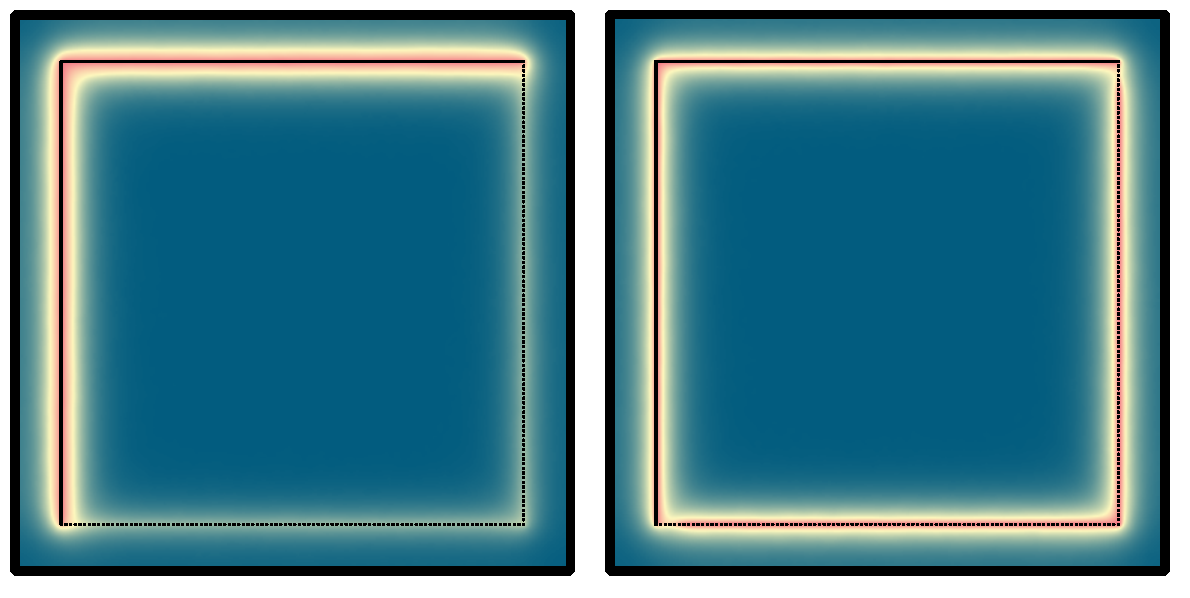
\includegraphics[width=0.95\textwidth]{Figures/2D_combined2.pdf}
    \caption{ Comparison of two heat solutions for a non-uniform 2D square-shaped point cloud (black dots). \textbf{Left:} Approximation of the heat solution using \emph{uniform weights} for the mean surface integral, \cref{standard_sum_heat}. \textbf{Right:} Solution using \emph{locally adaptive weights}, \cref{weighted_sum_heat}. The uniform weighting fails to maintain constant values along the zero-level set (see bottom left and top right corners), resulting in poorly oriented normals in regions with varying point density. This artifact is significantly reduced when using locally adaptive weights.}
    
\label{heatweights}
\end{figure}In practice, the surface $\S$ is given by a point cloud $\{x_i^\S\}_i\subsetneq\mathcal S$. This requires a transition from the integral term towards a discrete sum; if the input points are  uniformly distributed on $\S$, one could approximate
\cref{cont_functional} by \begin{align}\label{standard_sum_heat}
    \frac{1}{\S}\int_\S u\,\mathrm{da}\approx \frac{1}{N_{pt}}\sum_{i = 1}^{N_{pt}} u(x_i).
\end{align}
However, for the general case of a non-uniform point cloud, this approximation fails to recover reliable normal information, see \cref{heatweights} (left). Instead, we propose the following strategy to define a weighted sum approximating the integral: Let $\nu:\R^3 \rightarrow\R$ be a compactly supported, nonnegative, and smooth function. In practice, we take $$\nu(s) \coloneqq \begin{cases}
    \exp\Big(\frac{1}{|s|^2 - 1}\Big) &|s|<1.\\
    0  &\text{else.}
\end{cases}$$
We further define an $\epsilon$-scaled function $\nu^\epsilon \coloneqq \frac{1}{\epsilon ^3}\nu\big(\frac{s}{\epsilon}\big)$, $\epsilon \in \R^+$, which allows us to define the locally adaptive weights $\omega^\epsilon$ as follows:
$$\omega_i^\epsilon\coloneqq \frac{\tilde{\omega}_i^\epsilon}{\sum_i\tilde{\omega}_i^\epsilon}, \quad \text{where } \tilde{\omega}_i^\epsilon\coloneqq \Bigg(\sum_{j=1}^{N_{pt}}\nu^\epsilon(\|x_i^\S-x_j^\S\|)\Bigg)^{-1}.$$
The parameter $\epsilon$ controls the width of the support of $\nu^\epsilon$; thus, in our setting, it controls the size of the region around each point \( x_i^{\mathcal{S}} \) that contributes to the evaluation. In practice, we choose $\epsilon$ such that$$\forall\, i \leq N_{pt}:\quad\#\{\,x_j \text{ , s.t. } \|x_i^\S - x_j^\S\| < \epsilon\,\} > 12.$$ 
We obtain the approximation: 
\begin{align}\label{weighted_sum_heat}
    \frac{1}{\S}\int_\S u\, da\approx \sum_{i=1}^{N_{pt}}\omega_i^\epsilon\, u(x_i^\S).
\end{align}
For a visual comparison between uniform and adaptive weights, see \cref{heatweights}.
\paragraph{SDF step -- Inside/Outside regions:}
\begin{figure}[!b]
    \centering
    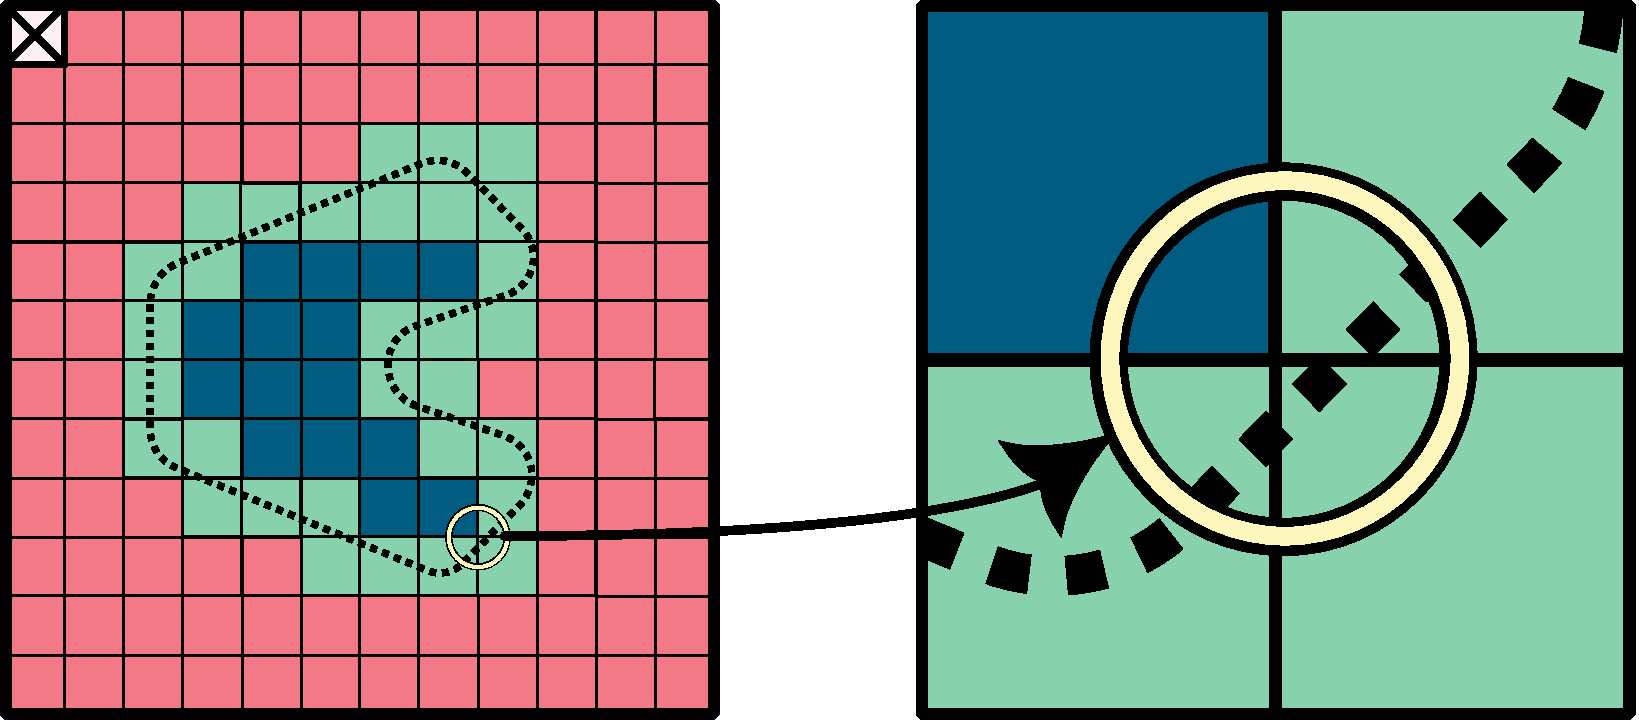
\includegraphics[width = 0.95\textwidth]{Figures/InnerOuter.pdf}\label{InnerOuter}
    \caption{\textbf{Left:} Visualization of the regions outputted by the box grid algorithm (\emph{without} dilation, step (ii)). The inner region (blue), outer region (red), and occupied cells (green) are shown together with the input point cloud (dashed line). The flood fill (step (iii)) is initialized from an outer region cell (marked with an "X"). We here point out that inner and outer regions may lie arbitrarily close to the point cloud (\textbf{right)}, which is why we dilate the region in step (ii).
}
\end{figure}
To ensure that the minimization process yields an SDF rather than an \emph{unsigned} distance function, we approximate the sets $\mathcal{B}^+$ outside and $\mathcal{B}^-$ inside the surface $\mathcal{S}$ using the following simple algorithm.
\begin{algorithm}\textbf{(Box-grid algorithm:)}\label{box_algorithm}
\begin{enumerate}
    \item Consider $\alpha \in \mathbb{Z}^3\cap h^{-1}\Omega$ and let $h\alpha $ be the cell midpoints of a rectangular grid with edge length $h > 0$. Iteratively mark all cells that contain at least one input point $x_i^\S$; these cells will be referred to as \emph{occupied cells}. In practice, we use $h = 64$ as the standard setting. For sparse input data, we recommend using smaller values, e.g. $h = 48$.
    \item By marking all direct neighbors of the occupied cells, we dilate the occupied region once. This introduces a safety distance between inside and outside regions and will be helpful later. For simplicity, we will here refer to the union of dilated and occupied cells as \emph{occupied region}. We will later use the occupied region to derive an effective sampling strategy in \cref{clever_sampling}.
    \item Next, starting with a cell that touches the boundary of $\Omega$ and is not in the occupied region, mark all neighbor cells that have not already been marked yet as \emph{exterior cells}. These cells define the set $\mathcal{B}^+_h \approx \mathcal{B}^+$.
    \item Finally, all cells that have not yet been marked will be marked as \emph{interior cells}, i.e., those defining the set $\mathcal{B}_h^-\approx \mathcal{B}^-$.
    \end{enumerate}
\end{algorithm}
\begin{remark}
    This simple and yet effective algorithm performs well for most commonly used examples in surface reconstruction. However, it may fail in certain situations; possible examples are input point clouds with surface holes, where the diameter of the missing part is bigger than the box diameter $h$. The algorithm is also not usable for layered surfaces, e.g., two spheres of different radii, where one is fully contained within the other.
\end{remark}
    In cases where our algorithm fails, we recommend the following strategy: 
    \begin{algorithm}\label{improvedInsideOutside}\textbf{(Improved inside/outside segmentation:)}
        \begin{enumerate}
            \item First, orient the point cloud by estimating surface normals, e.g., using the work from \cite{Metzer_2021}. They use a neural network to first learn coherent normal directions within individual patches of the point cloud and then orient the normals using a dipole propagation method. 
            \item In a second preprocessing step, we use the normals from step (i) to compute generalized winding numbers for a large number of sample points $z_i\in \Omega$. With generalized winding numbers, one can effectively segment the inner volume of complex shapes, even in the presence of self-intersections and non-manifold edges, see \cite{10.1145/2461912.2461916}.
            \item Finally, we can start the SDF training using batch-wise samples of the preprocessed points as $\mathcal{B}^\pm$ input.
        \end{enumerate}
    \end{algorithm} 
 
    For a visual comparison illustrating the limitations of the box-based algorithm and the effectiveness of the winding number method, see \cref{Winding_fig}
\begin{figure}[!t]
    \centering
    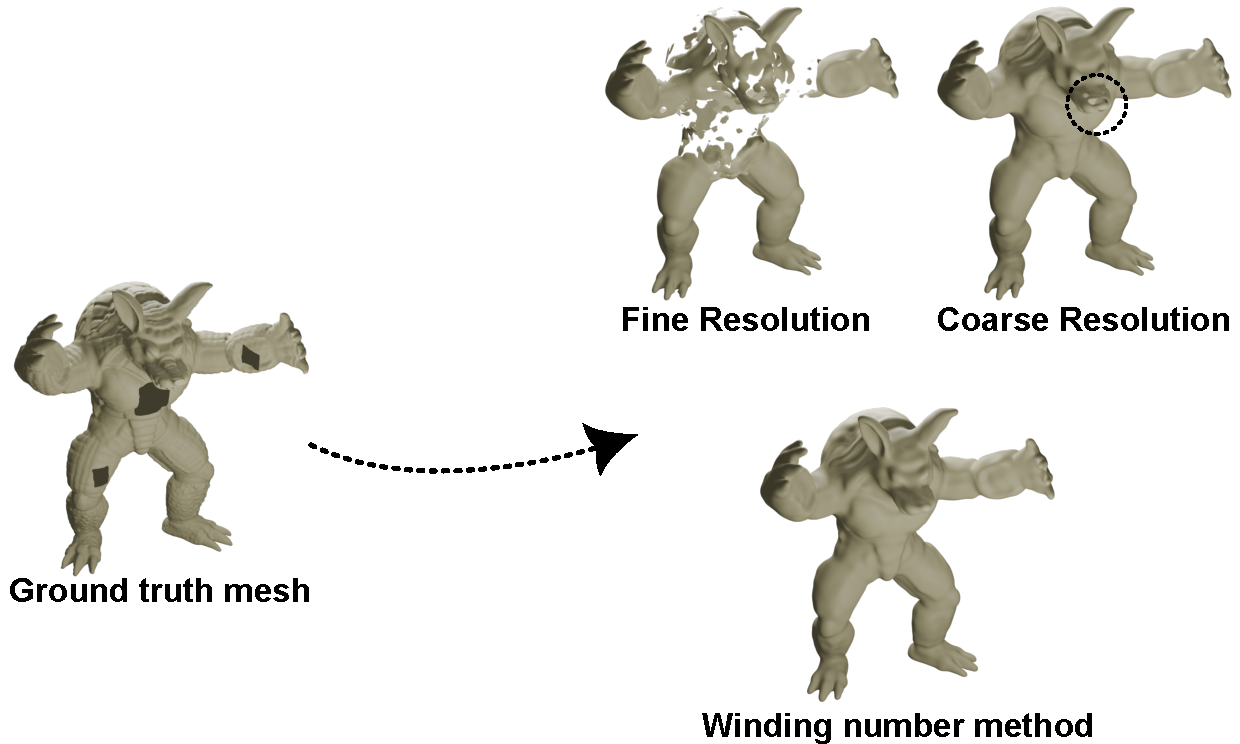
\includegraphics[width=\linewidth]{Figures/WindingNumberFig.pdf}
    \caption{We present results on an armadillo mesh with cut-outs using adaptations of the HeatSDF method. \textbf{Top:} Results obtained using our box-based algorithm (\Cref{box_algorithm}) for box sizes $h \approx 0.15$ and $h \approx 0.05$. While the larger box size (\textbf{top right}) yields reasonable segmentation, but produces small defects in narrow regions where no interior points are captured (highlighted by the dashed circle), the smaller box size (\textbf{top left}) leads to failures in distinguishing inside from outside. \textbf{Bottom:} Extracted zero-level set using the winding number method (\Cref{improvedInsideOutside}).
}
    \label{Winding_fig}
\end{figure}
\paragraph{SDF step -- Integration and sampling:} To evaluate the loss functional, we need to numerically approximate the integrals; we will do this via weighted sums. Then the functional $\mathcal{E}_{SDF}$ becomes
\begin{align*}
    \mathcal{E}_{SDF}(\phi) &\approx 
 \frac{1}{N_{pt}}\sum_{i=1}^{N_{pt}}\phi\big( x_i^\S\big)^2\\ &+ \frac{1}{N_{bs}}\sum_{i=1}^{N_{bs}}
\chi_{\{\phi < 0\}} \|\nabla \phi(x_j) + n_\tau(x_j)\|^2 + \chi_{\{\phi \geq 0\}} \|\nabla \phi(x_j) - n_\tau(x_j)\|^2  \\&+\frac{1}{N_{bd}} \sum^{N_{bd}}_{k = 1}\chi_{\{\phi(z^{out}_k) > 0\}} + \chi_{\{\phi(z^{in}_k) < 0\}}.
\end{align*}
Here, $N_{pt}\in \mathbb{N}$ is the number of input points $x_i^\S \in \mathcal S$;  $N_{bs}\in \mathbb{N}$ is the number of uniform samples $x_i$ inside the computational domain $\Omega$ and $N_{bd}\in \mathbb{N}$ is the number of samples $z^{out}, z^{in} \in \mathcal{B}_h^\pm$ inside and outside the surface, obtained by using the box-based algorithm, see \cref{box_algorithm}. In practice, we use $N_{bs} = 5000$ and $N_{bd} = 500$.\par
If one wants to solve for an SDF inside the whole domain $\Omega$, without taking into account the shape of $\S$, one can simply sample $x_j$ uniformly inside the whole computational domain. However, in some applications, for example in the context of narrow-band methods (see \cref{NPDEsonSurfaces}), one might only be interested in high-quality SDF approximations close to the surface. For this, we can adapt and extend the box-based algorithm described above to receive an effective yet simple sampling strategy that samples points uniformly inside the occupied region.
\begin{algorithm}\label{clever_sampling}\textbf{(Box-based near-surface sampling:)}
  \begin{enumerate}
      \item We first ensure that the sampling region has a certain width $\epsilon > 0$. We achieve this by iteratively repeating step (ii) from \cref{box_algorithm} for a total of $k = \lceil \frac{\epsilon}{h} \rceil$ times; that is, we mark direct neighbors of occupied cells as occupied. Let now $\mathcal{O}$ be the set of box midpoints of the occupied region after $k$-dilation steps. 
      \item We then uniformly sample $N_{bs}$ points $\{s_i\}$ inside the unit cube $[-1,1]^3$ and randomly choose $N_{bs}$ cell midpoints $\{m_i\}_{i \leq N_{bs}} \subset \mathcal O$.
      \item Let $\forall\, i \leq N_{bs}: \,x_i \coloneqq m_i + \frac{h}{2}\,s_i$. These evaluation points $x_i$ are uniformly distributed inside the dilated region.
  \end{enumerate}  
\end{algorithm}
\paragraph{SDF step -- Smoothed characteristic functions:} Due to the thresholding operations $\chi_{\{\phi<0\}}$ and $\chi_{\{\phi\geq 0\}}$, the functional $\mathcal E_n$ depends on the sets $\{\phi<0\}, \{\phi\geq0\}$ in a non-smooth manner, making the functional non-differentiable. This may cause problems during the optimization process. We overcome this issue by approximating the characteristic function $\chi$ using a smooth step-function depending on a small parameter $\delta \in \mathbb R^+$:
$$\eta_\delta(s) \coloneqq \eta\Big(\frac{s}{\delta}\Big), \quad \eta(s) \coloneqq
    \begin{cases}
1 & \text{if } s < -1 \\
\frac{1}{4} (s+2)(s-1)^2 & \text{if } |s| \leq 1 \\
0 & \text{if }s > 1
\end{cases}
$$
Notice that $\eta$ blends $C^1$-smooth between 0 and 1. Further, note that for $\delta \rightarrow 0,$ the convergence $\eta_\delta(s) \rightarrow\chi_{\{s<0\}}$ holds.\\
We can then approximate $\mathcal E_n$ by the smoothed functional $\hat {\mathcal{E}}_n$, given by
$$\hat{\mathcal E}_n(\phi) \coloneqq \int_\Omega \eta_\delta(\phi)\|\nabla \phi + n\|^2 + \big(1 - \eta_\delta(\phi)\big)\|\nabla \phi - n\|^2 \, \mathrm{d}x.$$
We further denote its discrete counterpart by $\mathcal{L}_n$, $$\mathcal L_n(\phi) \coloneqq \frac{1}{N_{bs}}\sum_j^{N_{bs}}
\eta_\delta(\phi) \|\nabla \phi(x_j) + n_\tau(x_j)\|^2 + \big(1 - \eta_\delta(\phi)\big) \|\nabla \phi(x_j) - n_\tau(x_j)\|^2.$$\\
We apply the same strategy to the boundary functional: 
\begin{equation}\label{eq:bd_functional}
    \mathcal{E}_{bd}(\phi) \approx \int_\mathcal{B^+} \eta_\delta(\phi) \,\mathrm{d}x + \int_{\mathcal{B^-}}(1-\eta_\delta(\phi)) \,\mathrm{d}x,
\end{equation}
and denote its discrete counterpart by $\mathcal{L}_{bd}$.\\
Note that in fact, $\forall\, \delta < h$, where $h$ denotes the edge length of the boxes, and $\mathcal{B}_h^{\pm}$ are the box regions obtained by using \cref{box_algorithm}, and for an SDF $\phi$, equality holds in \cref{eq:bd_functional}:
 $$\int_{\mathcal B^-}\chi_{\{\phi < 0\}}\,\mathrm{d}x + \int_{\mathcal B^+}\chi_{\{\phi > 0\}} \,\mathrm{d}x = \int_{\mathcal{B}^{-}_h} \eta_\delta(\phi) \,\mathrm{d}x + \int_{\mathcal{B}^{+}_h}(1-\eta_\delta(\phi)) \,\mathrm{d}x.$$
This is due to the safety distance we introduced in step (ii) of \cref{box_algorithm}. 
\paragraph{SDF step -- Far-field:}
\begin{figure}
    \centering
    \begingroup
    \sffamily  % ← switch to sans-serif font (Helvetica in pdfLaTeX)
    \def\svgwidth{\textwidth}
    \import{Figures/}{FarfieldvsNearfield.pdf_tex}
    \endgroup
    \caption{Comparison of our approach (HeatSDF) \emph{without far-field} (\textbf{left}) and \emph{with far-field} (\textbf{right}) on a 2D uniform box-shaped point cloud. We show both the SDF isolines at spacing 0.05 (\textbf{top}) and the gradient norm (\textbf{bottom}). In all plots, the reconstructed zero-level set is emphasized with a thicker black contour.}\label{farfield_comp}
\end{figure}
The solution of the heat step for small time $\tau$ yields reliable normal information within a narrow band around the surface. However, farther away from the surface, the heat solution approaches zero; consequently, the approximated gradient directions typically become unreliable due to oscillations, which prevents the computation of high-quality SDF normals in these regions. To address this problem, our method can be extended to produce accurate SDF approximations over large domains. This is achieved by solving an additional heat step for a larger time $\hat{\tau}$, in addition to the solution at time $\tau$, $\hat \tau >> \tau$. While being less accurate near the surface due to smoothing effects, the solution at the time step $\hat \tau$ provides stable gradient directions in regions farther away from the surface. In principle, this process could be repeated with multiple larger time steps $\hat{\tau}_k$, with $\hat{\tau}_i < \hat{\tau}_j$ for $i < j$, thereby progressively extending the reliable reconstruction domain. Using this technique, we can approximate SDFs inside arbitrary bounded subsets of $\R^3$.\\
For simplicity, assume for now that $k = 1$; we then adapt the functional towards 
\begin{align*}
    \mathcal{E}_n (\phi)&= \int_\Omega \eta_\delta(\phi)\, \|\nabla \phi + n_{blend}\|^2 + \big(1 - \eta_\delta(\phi)\big)\,\|\nabla \phi - n_{blend}\|^2 \,\mathrm{d}x\\  n_{blend} &= \beta^\tau(u_\tau)\, \nabla n_\tau + \big(1-\beta^\tau(u_\tau)\big)\,\nabla n_{\hat \tau}, \quad n_{\tau/ \hat \tau} = \frac{\nabla u_{\tau/ \hat \tau}}{\|\nabla u_{\tau/ \hat \tau}\|}, \\\beta^\tau(z) &= \begin{cases}
0 & \text{if } z < 0. \\
-2\,\big(\frac{z}{\kappa}\big)^3 + 3\, \big(\frac{z}{\kappa}\big)^2 & \text{if } 0 \leq \frac{z}{\kappa} \leq 1. \\
1 & \text{if } \frac{z}{\kappa} > 1.
\end{cases}
\end{align*} 
In practice, we use $\kappa = \frac{3}{5} \max_\Omega u_\tau $. Since the approximation of $u_\tau$ takes significantly less time compared to the SDF step, the far-field approach provides an easy way to approximate high quality SDFs on large domains.\par
For a visual comparison between the classical approach and the far-field approach, see \cref{farfield_comp}. 
\subsection{Method Summary}\label{ch:methodsummary} 
Using the implementation details presented in \cref{section_SDFmethod}, we construct the following two methods.
\paragraph{HeatSDF:} First, let us define the method \emph{HeatSDF} (\cite{weidemaier2025sdfsunorientedpointclouds}); HeatSDF uses smoothed characteristic functions to approximate the normal loss. To extend the global quality of the SDF, we compute two time steps of the heat flow, $\tau = 0.005$ and $\hat \tau = 0.1 $. The integrals are evaluated using uniform points inside the whole domain $\Omega$.
\begin{align}
    &\mathcal{L}_{HeatSDF}(\phi) \coloneqq \lambda_1\, \mathcal{L}_{surf}(\phi) + \lambda _2\,\mathcal{L}_{n}(\phi) + \lambda_3\,\mathcal{L}_{bd}(\phi)\notag \\
    &\quad =\frac{\lambda_1}{N_{pt}}\sum_{i=1}^{N_{pt}}\phi\big( x_i^\S\big)^2
     \notag\\\displaybreak[1]\notag & \quad + \frac{\lambda_2}{N_{bs}}\sum_{j = 1}^{N_{bs}}
\eta_\delta(\phi) \|\nabla \phi(x_j) + n_{blend}(x_j)\|^2 + \big(1 - \eta_\delta(\phi)\big) \|\nabla \phi(x_j) - n_{blend}(x_j)\|^2 \notag\\ & \quad+ \frac{\lambda_3}{N_{bd}} \sum_{k = 1}^{N_{bd}} \eta_\delta\circ\phi(z_k^{out}) +\big(1-\eta_\delta\circ\phi(z_k^{out})\big) 
\end{align}
As a default setting, we choose $\lambda_1 = 100, \,\lambda_2 = 1, \,\lambda_3 = 1$, and use $\delta = 0.005$. The parameter $\lambda_1$ controls the trade-off between surface details and gradient quality. We set $\lambda_1 = 100$ to prioritize high-quality gradients while still maintaining descent surface reconstruction.
\paragraph{NeatSDF:} Furthermore, we can define an improved version, called \emph{NeatSDF}. NeatSDF approximates the SDF inside a narrow band region $D$, such that \mbox{$\S\subsetneq D\subsetneq\Omega,$} using the sampling strategy defined in \cref{clever_sampling}. In addition to the standard loss terms $\mathcal{L}_{surf}, \mathcal L_{n}$, and $\mathcal{L}_{bd}$, we add the singular Hessian term 
$$ \mathcal L_{Hess}(\phi) \coloneqq \int_\Omega |\det(D^2 \phi(x))| \,\mathrm{d}x + \epsilon_{Hess} \|\phi \|_{W^{2,p}}^p. $$ The regularization of the Hessian term in normal direction allows us to slightly adapt the normal loss:
\[\tilde{\mathcal{E}}_{n}(\phi)= \int_D \min(\|\nabla \phi + n\|^2,\|\nabla \phi - n\|^2) \,\mathrm{d}x.\]
Note that $\tilde{\mathcal{E}}_n$ is not weakly lower semicontinuous. To recover lower semicontinuity, one could approximate the $\min(\cdot,\cdot)$ by a smooth function $\min(\epsilon;a,b) \coloneqq \frac{a + b}{2} - \frac{1}{2}\sqrt{(a-b)^2 + \epsilon}$, where $ \min(\epsilon;a,b) \xrightarrow[]{\epsilon \rightarrow0} \min(a,b).$ In this case the functional $\tilde {\mathcal E}^\epsilon_n$ including $\min(\epsilon; \,,\,)$ is weakly lower semicontinuous for all $\epsilon > 0$. We omit the proof here and refer to the Appendix (\Cref{min_lsc}). Since our experiments did not indicate any convergence issues, we retain the \mbox{$\min$- operator} in practice.\par
The overall loss function for the NeatSDF method reads \begin{align}
    &\mathcal{L}_{NeatSDF}(\phi) \coloneqq \lambda_1\, \mathcal{L}_{surf}(\phi) + \lambda _2\,\hat{\mathcal{L}}_{n}(\phi) + \lambda_3\,\mathcal{L}_{bd}(\phi) + \lambda_4\, \mathcal{L}_{Hess}\notag\\
    &\quad =\frac{\lambda_1}{N_{pt}}\sum_{i=1}^{N_{pt}}\phi\big( x_i^\S\big)^2
     \notag\\\notag & \quad + \frac{\lambda_2}{N_{bs}}\sum_{j=1}^{N_{bs}}
\min\big( \|\nabla \phi(x_j) + n_\tau(x_j)\|^2, \|\nabla \phi(x_j) - n_\tau(x_j)\|^2\big) \notag\\\displaybreak[1]
& \quad+ \frac{\lambda_3}{N_{bd}} \sum_{k=1}^{N_{bd}} \eta_\delta\circ\phi(z_k^{out}) +\big(1-\eta_\delta\circ\phi(z_k^{out})\big)\notag\\
&\quad +\frac{\lambda_4}{N_{bs}}\, \sum_{j=1}^{N_{bs}}|\det\big( D^2 \phi(x_j)\big)| + \epsilon_{Hess}\Big[\,|\phi|^p + \|\nabla \phi\|^p + \left( \sum_{l=1}^d \| \partial_l \nabla \phi \|^2 \right)^{p/2} \,\Big](x_j) .
\end{align} 
As a default parameter setting, we use $\lambda_ 1 = 10^5, \,\lambda_2 = 10, \,\lambda_3 = 100, \,\lambda_4 = 10^{-6}$, which has proven to be a good trade-off between highly accurate surface reconstruction and reliable SDF gradients. The method is stable with respect to variations in the parameter settings.\par
Note that other combinations of the functionals are possible. For example, one could use the NeatSDF method with the far-field approach or use the HeatSDF method with near-surface sampling. 
\section{Experiments and Comparison}\label{Comps}
The theoretical framework presented above is directly adaptable to work in dimension $n=2$, see, for example, the results in \cref{heatweights,farfield_comp}. In the following, we restrict our attention to examples based on three-dimensional point clouds, as this case is more challenging to compute, and thus provides a more rigorous test of the methods. Building on the theory presented above, we defined two loss functionals in \cref{ch:methodsummary}, whose minimizers approximate SDFs corresponding to the input surface. We compare these approaches with the following state-of-the-art methods; note that to improve readability, we do not explicitly include the scaling factors between the loss terms.
\paragraph{SALD, \cite{SALD}:} This approach extends the original \emph{Sign Agnostic Learning (SAL)} framework, \cite{SAL}, by incorporating derivatives into the loss functional. SAL learns an SDF from unoriented input data via a loss functional that compares discrete point-wise distances up to unknown sign:
$$L_{SAL}(\phi) \coloneqq \int_\Omega\big||\phi(x)| - \min_{i} \mathrm{d}( x_i^\S, x)\big|\,\mathrm{d}x.
$$
They reconstruct a \emph{signed} distance function by utilizing an initialization based on the unit sphere.
SALD improves the SAL method by including point-wise derivatives:
$$L_{SALD}(\phi) \coloneqq L_{SAL}(\phi)\, +\, \int_\Omega \min \|\nabla\big(\min_{i} \mathrm{d}( x_i^\S, x)\big) \pm \nabla \phi(x)\|  \,\mathrm{d}x.$$
Both SAL and SALD use ReLU activation functions.

\paragraph{HESS, \cite{wang2023neuralsingularhessianimplicitneuralrepresentation}:} This method builds on the basic \emph{SIREN} SDF-framework by \cite{sitzmann2020implicitneuralrepresentationsperiodic}:
$$
L_{SIREN}(\phi) \coloneqq \int_\S |\phi| + (1-n\cdot\nabla \phi) \,\mathrm{da} + \int_\Omega \big|\|\nabla \phi\| - 1\big| \,\mathrm{d}x + \int_{\Omega\setminus\S} \exp(-\alpha |\phi|) \,\mathrm{d}x,
$$
for some $\alpha >> 1$. Here, $n$ denotes the ground truth surface normal field, thus SIREN requires oriented input data.\\
Similarly, the HESS method reads
$$L_{HESS}(\phi) \coloneqq \int_\S |\phi| \,\mathrm{da} + \int_\Omega \big|\|\nabla \phi\| - 1\big|  + |\det(D^2\phi)| \,\mathrm{d}x + \int_{\Omega\setminus\S} \exp(-\alpha |\phi|) \,\mathrm{d}x. $$
By incorporating the singular Hessian term, they enforce regularity of the SDF in normal direction, allowing to reconstruct surfaces from unoriented point clouds. \\
During training, the authors iteratively reduce the contribution of the Hessian term by decreasing its weighting. This process allows to recover highly detailed zero-level sets. It is important to note that the exponential damping term fundamentally limits the method’s ability to approximate accurate off-surface distances. However, the main focus of the methods seems to be on surface reconstruction rather than SDF properties. The method is flexible with respect to the activation functions, but achieves best results using the SIREN activation. 
\paragraph{1-Lip, \cite{1lip}:} The proposed method ensures that the neural function is 1-Lipschitz, meaning it cannot overestimate distances. To this end, the authors use a special network architecture proposed by \cite{araujo2023unifiedalgebraicperspectivelipschitz}. The 1-Lipschitz property of the whole network is here achieved by designing network layers with Lipschitz constant $L=1$, as the Lipschitz constant of a composition is upper bounded by the product of all Lipschitz constants.\\
Then, they use a loss function from optimal transport, that maximizes distance values to off-surface points over all 1-Lipschitz functions. More precisely, they use the \emph{hinge-Kantorovich-Rubenstein} loss, 
$$
L_{1Lip}(\phi) \coloneqq \int_\Omega (\chi_{\mathcal B^-}-\chi_{\mathcal B^+})(x)\,\phi(x)  + \max\big(0,m+ (\chi_{\mathcal B^-}-\chi_{\mathcal B^+})(x)\phi(x)\big)\,\mathrm{d}x,
$$
with $\lambda,m >0$ and $\mathcal{B}^\pm$ being the given sets on the inside and outside of $\S$. The first part of the integral is the dual formulation of the Wasserstein-1 distance. The second term  penalizes points for which the sign of $\phi$ does not match the sign of $ (\chi_{\mathcal B^-}-\chi_{\mathcal B^+})$. The parameter $m$ acts as a threshold; lower values of $m$ improve zero-level sets quality, but also makes the optimization less stable.\\
The method requires information on inside and outside of the surface; for this, the authors use an approach based on generalized winding numbers, similar to \cref{improvedInsideOutside}. Their implementation uses ground truth normals to compute the generalized winding numbers, leaving it unclear if approximated normals would suffice. Their main focus seems to be on accurate distance estimation.
\paragraph{HotSpot, \cite{hotspot}:} The model is based on the screened Poisson equation, which reads

$$u(x) - t\,\Delta u(x) = 0 \text{ on } D\subset \R^n, \quad u = 1 \text{ on } \partial D,$$
and its relation to distances via Varadhan's formula (\cite{varadhan}):
$$
\lim_{t\rightarrow0} \sqrt{t}\ln(1/u(x)) = \mathrm{d}(x),$$ 
where $\mathrm{d}$ denotes the distance to the boundary of the domain $D$. To approximate SDFs, the authors introduce a heat-based loss $$L_{heat}(\phi) = \frac{1}{2}\int_\Omega e^{-2\lambda |\phi(x)|}\big(\|\nabla \phi(x)\|^2 + 1\big) \,\mathrm{d}x.$$ Taking the derivative with respect to the heat field $h(x) = e^{-\lambda|\phi(x)|}$ recovers the screened Poisson equation. Their overall loss reads $$L_{HotSpot}(\phi) = \int_\S |\phi|\,\mathrm{da}  + \int_\Omega \big|\|\nabla \phi\| - 1\big|\,\mathrm{d}x + L_{heat}(\phi).$$
During training, the individual scaling factors in front of the integrals change, depending on a complex routine established by the authors.\\ 
While being similar to our approach due to its connection to the heat equation, the method still depends on the Eikonal equation, making it non-convex and not well-posed.
\subsection{Evaluation Metrics}
To evaluate the quality of the SDF methods, we choose different metrics that measure both the quality of surface reconstruction (\(\mathbf{E_{recon}^{\mathcal{S}}}\), $\mathbf{E_{recon}^n}$) and the SDF quality, taking into account the Eikonal error ($\mathbf{E_{eik}}$), and the distance quality ($\mathbf{E_{SDF}}$) inside a narrow band. Our experiments use point clouds generated from meshed surface geometries, providing ground truth surface data.
\begin{enumerate}[align=left]
\item[\(\mathbf{E_{recon}^{\mathcal{S}}}:\)]  The squared $L^2$-error evaluated on the set $\mathcal M$, with $\#\mathcal M = 50.000$ distinct ground truth on-surface points sampled from the meshed input surface to measure the reconstruction error.
 $$\mathbf{E_{recon}^{\mathcal{S}}}\coloneqq\frac{1}{\# \mathcal{M} }\sum_{x \in \mathcal{M}} \phi(x)^2.$$
\item[$\mathbf{E_{recon}^n:}$] The $L^1$-cosine distance between the gradients of the SDF on the zero-level set and the normals of the mesh. Here, $n(x)$ denotes the discrete normal of the triangle midpoint $x$ of the ground truth mesh and $\mathcal{F}$ is the set of face centers. 
$$\mathbf{E_{recon}^n} \coloneqq1 - \frac{1}{\#\mathcal{F}} \sum_{x\in \mathcal{F}} n(x)\cdot\frac{\nabla  \phi(x)}{\|\nabla \phi(x)\|}. $$
\item[$\mathbf{E_{SDF}:}$] The $L^1$-error between the learned SDF and the ground truth signed distance on a total of $\#\mathcal N = 10.000$ uniformly distributed points $x$ inside a narrow band $\mathcal{N}$ with $|\mathrm{d}(x, \mathcal{S})| < 0.1$, for all $ x\in \mathbb N$.
$$\mathbf{E_{SDF}} \coloneqq \frac{1}{\#\mathcal{N}}\sum_{x\in \mathcal{N}}|\phi(x) - \mathrm{d}(x, \mathcal{S})|.$$% (if available, e.g., if the surface is given as a mesh). 
\item[\(\mathbf{E_{{eik}}:}\)] The median Eikonal error is evaluated within a narrow band around the surface, using the same set of points as for the SDF error evaluation.
 $$\mathbf{E_{eik}} \coloneqq \mathrm{median} \left\{x\in \mathcal{N} \, \mid\,  \big|\|\nabla\phi(x)\| - 1\big|\right\}. $$
\end{enumerate}
\subsection{Comparisons}
All examples are scaled such that they are fully contained in $[-1,\,1]^3$; we take $\Omega = [-1.2, \,1.2]^3$ as our computational domain to make sure that there is enough distance separating $\mathcal S$ and $\partial \Omega$. \\
We extend the experiments shown in \cite{weidemaier2025sdfsunorientedpointclouds}, comparing HeatSDF and NeatSDF with the previously discussed baseline algorithms for five example shapes (Planck head, Stanford bunny, hand, armadillo, lightbulb), see \cref{tab:handquant,fig:hand_vis,scatter_methods}. \\
Additionally, we present an experimental convergence result of the NeatSDF method on a simple geometry, \cref{convergence}. \\
Overall, the NeatSDF method outperforms the HeatSDF method for all examples; for a visual comparison, see \cref{Head_comp}. Compared to the other methods, only the HotSpot method is able to produce comparable results. We point out that our method is far more accurate than HotSpot with respect to the SDF distance.
\begin{figure}[t]
    \centering
    \begingroup
    \sffamily
    \def\svgwidth{0.95\textwidth}
    \import{Figures/}{Hand_Comparison.pdf_tex}
    \endgroup
    \caption{Qualitative comparison of all methods for the hand geometry.}
    \label{fig:hand_vis}
\end{figure}
\begin{figure}[b]
    \centering
    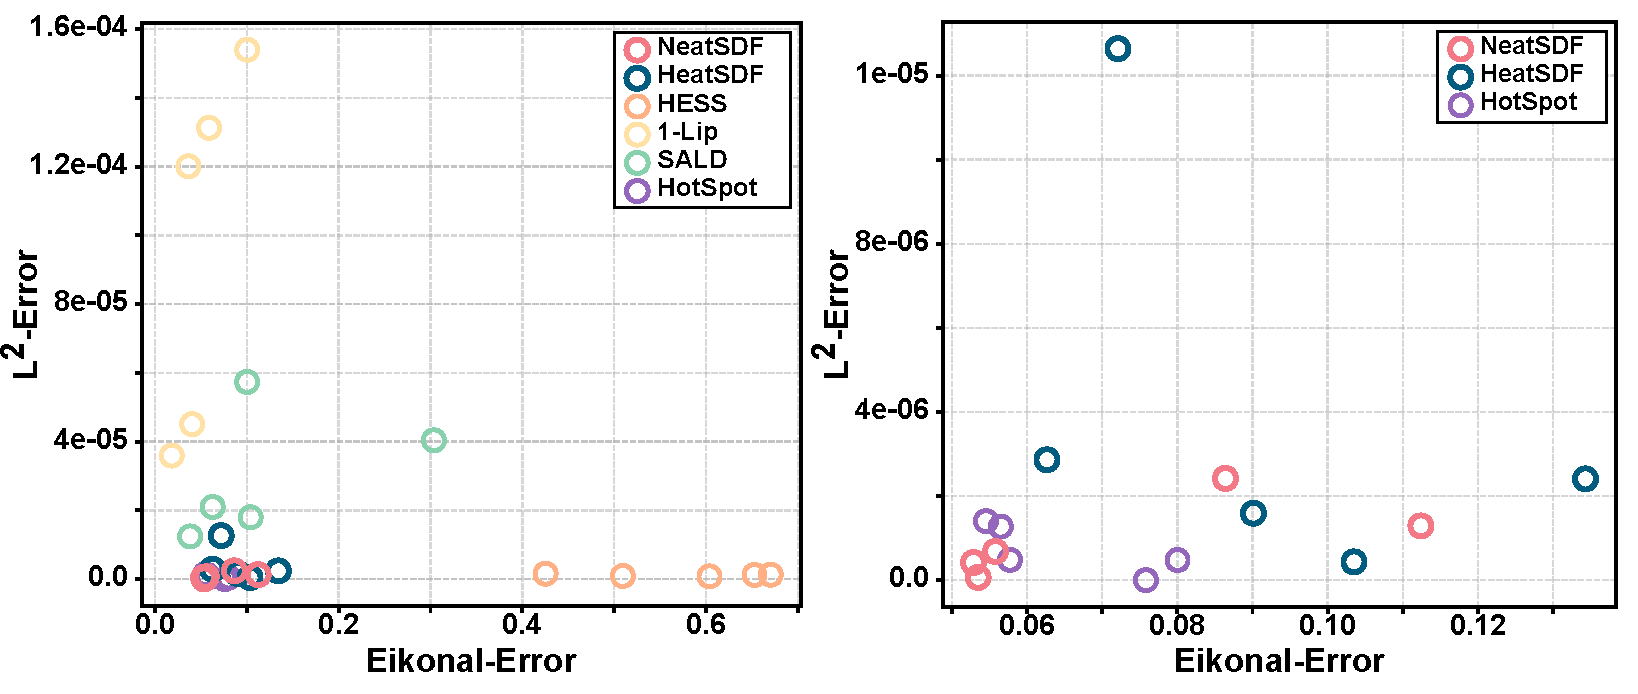
\includegraphics[width =0.99\textwidth]{Figures/method_comparison_lager_letters.pdf}
    
   
    \caption{Quantitative comparison of the $L^2$-surface error $\mathbf{(E_{recon}^{\mathcal{S}})}$ and Eikonal error $\mathbf{(E_{\text{eik}})}$ for five different shapes (Planck head, Stanford bunny, hand, armadillo, lightbulb) for all methods (\textbf{left}) and for the three methods with the best performance (\textbf{right}). While some methods show good results wrt. a single error metric (HESS for $L^2$-error, 1-Lip for Eikonal error), our methods yield results that are consistently close to the best overall for both metrics. HotSpot and NeatSDF yield similar errors.}  \label{scatter_methods}
\end{figure}



\begin{figure}
\hspace*{-0.3cm}
\includegraphics[width = \textwidth]{Figures/SDF_scatter_all3.pdf}
\vspace*{0.5cm}  % <-- add * to force spacing
    \par  % <-- force a paragraph break to make spacing take effect
        \begin{tabular}{cccccc}
        \toprule
        \textbf{Method} &$\mathbf{E_{recon}^{\mathcal{S}}}$ & $\mathbf{E_{eik}}$ &$\mathbf{E_{recon}^n}$ & $\mathbf{E_{SDF}}$\\ 
        \midrule
        SALD & 5.736e-05 &  0.1003 & 0.10630 & 0.01308\\ %0.05737\\  % hand   \\ 
        HESS & 1.268e-06  &  0.6704 &\textbf{0.00134} &0.02547   \\ 
        1-Lip   & 1.201e-04   & \textbf{0.0363} &0.03793&0.01981\\  % hand  \\ 
        HotSpot  &7.485e-07 &   0.0651 & 0.00152 &  0.02578\\  % hand
        \midrule
        HeatSDF & 1.591e-06  & 0.0901 &  0.00262&0.01184\\  % hands/NeuralSDFs3_2025-Mar-27-11-31-30
        
        NeatSDF & \textbf{4.984e-07} & 0.0576 & 0.00186 & \textbf{0.00337} \\%logs/SDF2025-Jun-13-12-12-25/SDF_step
        \bottomrule
    \end{tabular}
    \caption{\textbf{Top:} Scatter plots showing the the SDF values of all methods evaluated on the hand geometry. Other methods either struggle to approximate good distances for points away from the surface (HESS), show globally good consistency but tend to underestimate the distance (1-Lip), or demonstrate good consistency with a slight difference in the slope (HotSpot). Comparing our methods, NeatSDF outperforms HeatSDF for points far away from the surface. \textbf{Bottom:} Quantitative evaluation of all methods for the hand geometry.}
    \label{tab:handquant}
\end{figure}
% \begin{table}[t]
%     \centering
%         \begin{tabular}{ccccc}
%         \toprule
%         \textbf{Method} &$\mathbf{E_{recon}^{\mathcal{S}}}$ & $\mathbf{E_{eik}}$ &$\mathbf{E_{recon}^n}$ & $\mathbf{E_{SDF}}$\\ 
%         \midrule
%         SALD &2.10e-05&0.0628&0.03087&0.00754\\
%         HESS &7.92e-07&0.6038&\textbf{0.00070}&0.02464\\
%         1-Lip   &4.51e-05&\textbf{0.0404}&0.02765&0.01077\\
%          HotSpot  &4.74e-07&0.0763&0.00104&0.00760\\
%         \midrule
%         HeatSDF & 4.35e-07&0.1035&0.00149&0.01208\\
        
%         NeatSDF & \textbf{6.426e-08} & 0.0535 & 0.00078 & \textbf{0.00349} \\%logs/SDF2025-Jun-18-19-45-09/SDF_step
%         \bottomrule
%     \end{tabular}
%     \caption{Quantitative evaluation of all methods for the Stanford bunny.}
%     \label{tab:bunnyquant}
% \end{table}

\begin{figure}
    \centering
    \begin{minipage}[c]{0.7\textwidth}
        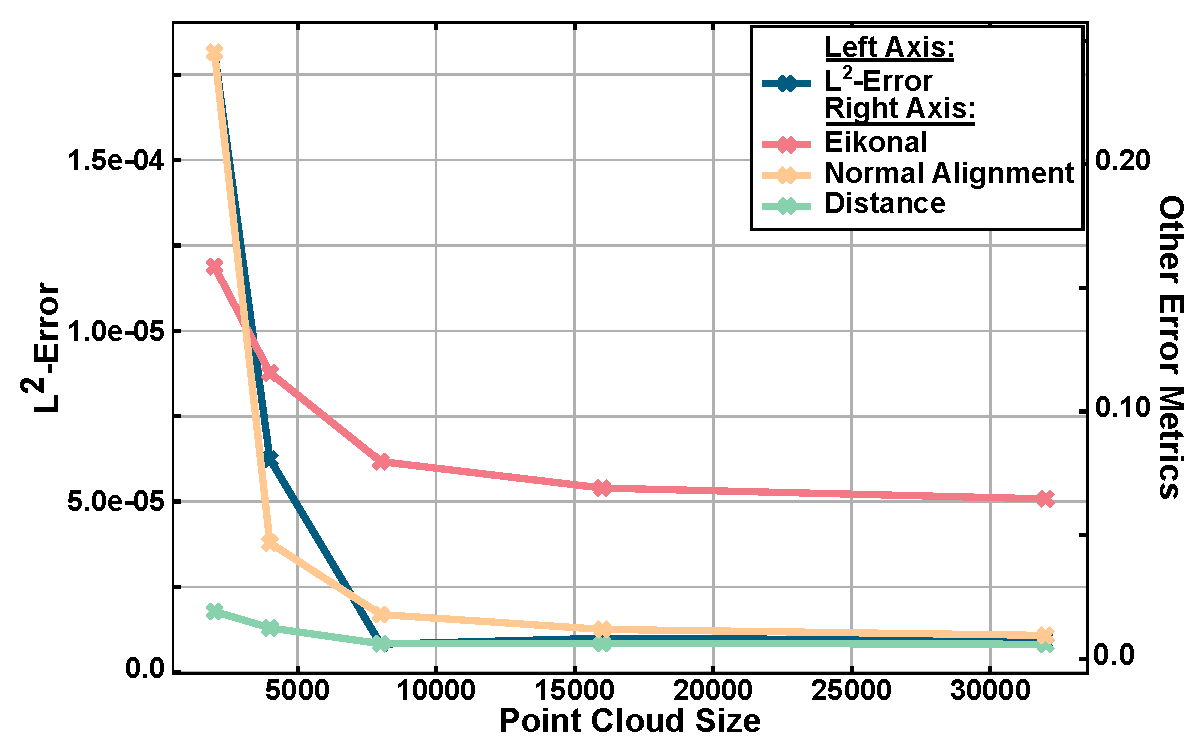
\includegraphics[width=\textwidth]{Figures/conv_vis.pdf}
    \end{minipage}%
    \hfill
    \begin{minipage}[c]{0.25\textwidth}
        \centering
        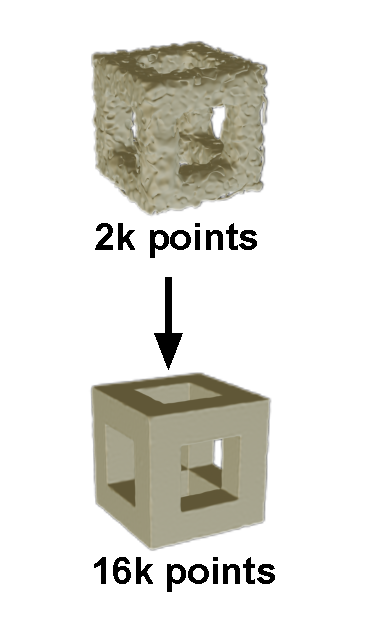
\includegraphics[width=\textwidth]{Figures/convergence_vert.pdf}
    \end{minipage}
    \caption{
\textbf{Left:} Quantitative evaluation on a cubical frame for different point cloud sizes. The errors decrease for all metrics as the number of input points increases. 
\textbf{Right:} Visualization of the extracted zero-level set for input point clouds of the cubical frame of size 2.000 and 16.000.}
\label{convergence}
    
\end{figure}

\begin{figure}
    \centering
    \begingroup
    \sffamily
    \def\svgwidth{0.90\textwidth} % or 0.8\textwidth, etc.
    \import{Figures/}{Head_Comparison.pdf_tex}
    \endgroup
    \caption{Qualitative comparison of the NeatSDF and HeatSDF method for the Planck head. The HeatSDF result loses most of the details compared to the input geometry; this effect is significantly reduced when using the NeatSDF method.}
    \label{Head_comp}
\end{figure}
\FloatBarrier

\subsection{Geometric Queries}

As a first application, we demonstrate that both HeatSDF and NeatSDF are sufficiently accurate to compute the intersection and union of the sublevel sets ${\phi_i < 0}$ for given SDFs $\phi_i$. For two SDFs $\phi_1$ and $\phi_2$, the union and intersection of their sublevel sets can be written as:
\begin{align*}
    \{\phi_1 < 0\} \cup \{\phi_2 < 0\} = \{\min\{\phi_1, \phi_2\} < 0\}. \\
    \{\phi_1 < 0\} \cap \{\phi_2 < 0\} = \{\max\{\phi_1, \phi_2\} < 0\}.
\end{align*}
However, note that in general neither the union nor the intersection of two SDFs yields another SDF. \Cref{intersAndunion} shows two examples.
\begin{figure}
    \centering
    \includegraphics[width = 0.95\textwidth]{Figures/UnionAndIntersection2.pdf}
    \caption{\textbf{Bottom:} Intersection of the Stanford bunny with a scaled and modulated pipe-like structure by computing the point-wise maximum. Both results on the left were computed using the HeatSDF method. \textbf{Top:} Union of a Beethoven sculpture with a pair of headphones by computing the point-wise minimum. Both results on the left were computed using the NeatSDF method.}\label{intersAndunion}
\end{figure}
\chapter{Neural PDEs on Neural Surfaces}\label{NPDEsonSurfaces} 
\paragraph{Motivation:} Partial differential equations play a central role in many areas of science and engineering, including image processing, fluid mechanics, and material science. In practice, these equations are naturally posed on manifolds rather than in flat space. A variety of methods have been proposed both for flat and curved domains; these include well-known methods such as the finite element and finite difference method. \par
Over the recent years, there has been growing interest in solving PDEs using neural networks, both from a theoretical and practical perspective. PDEs defined on flat domains in $\R^n$ have been extensively studied within neural network frameworks, using a variety of methods like PINNs or neural-variational formulations. However, the study of PDEs on manifolds using neural networks remains relatively underdeveloped. Most existing work focuses on specific geometries, predominantly the unit sphere, and considers only limited classes of PDEs.
To develop the area of geometric PDEs towards more general and flexible settings, one must first address how to represent the underlying manifold. Several possibilities come to mind, such as local charts, mesh-based representations, and point cloud approximations. One compelling approach is the use of SDFs. This representation enables the usage of narrow-band methods, which have proven successful in the classical (non-neural) setting for simulating surface evolution and solving geometric PDEs.
This thesis builds on these developments and extends them by studying how geometric PDEs can be formulated and solved on general implicit surfaces via neural networks.
\section{Related Work}
\paragraph{Neural PDEs on flat domains:}
The use of neural networks to solve partial differential equations was first proposed in the 1990s. For instance, \cite{Lagaris_1998} proposed to use feedforward architectures to approximate PDE solutions by minimizing residuals. These early approaches were conceptually promising but limited by computational resources and the lack of efficient training algorithms. A significant advancement occurred with the introduction of physics-informed neural networks (PINNs), see \cite{RAISSI2019686}, which embed PDE constraints directly into the loss function when working with data-driven networks. Although we are not interested in data-driven networks, the proposed concepts generalize easily to a pure mathematical context: A PINN in our sense minimizes the sum of squared PDE residual functions; for example, for the Poisson equation, $\Delta u = f$, we have: $$ \text{solve: }\,\Delta u = f \quad\rightarrow\quad \min_u \int_D|\Delta u - f| ^2 \,\mathrm{d}x.$$
\par
In contrast, the Deep Ritz method (\cite{deepritzmethoddeep}) is designed to solve variational problems, especially those arising from PDEs. In this method, the PDE is reformulated as an optimization problem of a variational functional. For the example above, this yields: $$\text{solve: } \,\Delta u = f\quad \rightarrow \quad\min_u \int_D \frac{1}{2}\|\nabla u\|^2 + fu \,\mathrm{d}x.$$
As mentioned above, variational neural approaches, such as the deep Ritz method, are particularly well-suited to our applications.
\par
Neural networks for solving PDEs offer several advantages over traditional grid-based methods, like finite element (FEM) or finite difference methods (FDM). Some of the key benefits are: \begin{itemize}
\item \textbf{Flexibility and smoothness:}
Neural networks are universal function approximators and can be used to approximate solutions to a wide class of PDEs. 
\item\textbf{Mesh-free nature:} Unlike FEM/FDM, which require meshing and are constrained by grid resolution, neural networks provide mesh-free approximations, enabling flexible handling of complex geometries and irregular domains.
\item \textbf{High-dimensional scalability:} Classical methods scale poorly with increasing dimension, due to the \emph{curse of dimensionality} (exponential growth in grid points). Neural networks can handle high-dimensional inputs more efficiently.
\end{itemize}
Although being beyond the scope of this thesis, we point out that the development of neural operators has opened new possibilities by learning mappings between infinite-dimensional function spaces. These operator-learning models enable fast, mesh-free solution generation (see, for example, \cite{li2021fourierneuraloperatorparametric} and \cite{Lu_2021}).
\paragraph{Neural geometric PDEs:}
Neural PDEs on flat domains have been extensively studied over the previous years. However, work regarding curved domains is limited to a few articles, all of which use the PINN approach; for example, \cite{tangfu} present some simple examples on 3-dimensional manifolds. Their work lacks generality because they discretize the surface once, before the beginning of the training procedure, and then use the same points throughout the  entire process. Furthermore, their quantitative error analysis is evaluated only on these precomputed training points, ignoring the global behavior of their solution entirely. In another paper, \cite{lei2024solvingpdesspheresphysicsinformed} proved an upper bound for the approximation error of geometric PINNs on the sphere and presented some experiments.\par
Both publications lack generality, as they are restricted to simple domains; this is an issue of the geometric PINN method itself, since (uniform) random sampling on manifolds might be difficult or impossible in general. Using a fixed set of points during the training process, on the other hand, neglects the mesh-free advantage of neural approaches. 
\paragraph{Discrete narrow-band methods:}
Traditionally, narrow-band methods have been used to solve PDEs in a narrow band around an implicitly defined surface. One discretizes the narrow-band domain by a mesh; a smooth cut-off function is used to blend near the boundary of the band. This approach allows effective handling of complicated geometries while maintaining computational efficiency (see, for example, \cite{deckelnick} and \cite{neRU}). We propose to lift classical narrow-band methods, as they have been used in combination with FEM and FDM, to a neural context. 
\section{Neural Narrow-Band Methods}
Let in the following $\phi$ be an SDF and let $\S$ be its zero-level set; further, consider the level sets $\mathcal{M}_c \coloneqq \{x\in \R^3 \text{ , s.t. } \phi(x) = c\}$ for $c \in \R$. Let $\nabla_{\mathcal{M}_c}$ and $\mathrm{div}_{\mathcal{M}_c}$ denote the tangential gradient and divergence with respect to the level set $\mathcal M_c$, and $\Delta_{\mathcal M_c} \coloneqq \mathrm{div}_{\mathcal{M}_c}\nabla_{\mathcal{M}_c} $ the Laplace-Beltrami operator.\par
Assume that we want to compute \begin{align}\label{level_set_mini}
    \min_{w\in \mathcal{C}^\infty}\int_{\mathcal{M}_c} F(w(x)) \,\mathrm{d}x,
\end{align} for some given function $F:\R^n \rightarrow\R$ and $w: \R^3 \rightarrow\R^n$. As mentioned above, a numerical approximation of this integral is difficult for general geometries $\mathcal M_c$, since generating random quadrature points on the level set might require preprocessing. \par
Instead, one can use the co-area formula, \cref{Co_Area_form}, allowing us to rewrite the surface integral over a family of level sets as a volume integral
$$\int_\R\int_{\mathcal{M}_c} F(w(x)) \,\mathrm{d}x\,\mathrm{dc}= \int_{\R^d}F(w(x)) \,\mathrm{d}x.$$
In practice, we will evaluate the integral in a narrow band around the zero-level set using a smooth cut-off function $\eta: \R\rightarrow\R$, with $\eta = 1$ for $[-\epsilon/2,\epsilon/2]$ and $\eta = 0$ on $\R \setminus(-\epsilon, \epsilon)$. Thus, instead of \cref{level_set_mini}, we consider: 
$$\min_w \int_{\R^d} \eta(\phi(x))\,F(w(x))  \,\mathrm{d}x.$$
The exact solution of the minimization problem decouples over all level sets, while the numerical approximation of the minimizers only provides an approximative decoupling.
We evaluate this integral numerically by using the box-sampling algorithm presented in \cref{clever_sampling}. For our present application, we must ensure that the minimum distance of $\S$ to the boundaries of the dilated region is larger than $\epsilon$, thus we dilate k-times, where $k = \Big\lceil\frac{\epsilon}{h}\Big\rceil,$
and $h$ denotes the edge length of the boxes. Then, we can uniformly sample inside the dilated box-region.
\section{Experiments}
We now employ the neural SDFs generated by the methods presented in \cref{section_SDFmethod} to solve geometric PDEs on the zero-level sets. In the absence of comparable neural methods, we evaluate our results against ground truth solutions, or those obtained via finite element methods.
\subsection{Geometric Poisson Problem}\label{section_PoissonPB}
Consider the geometric Poisson problem: \begin{equation}\label{Poisson_eq}
    -\Delta_{\mathcal{M}_c} u = f,\quad \text{ with }
    u,f: D \rightarrow \R, 
\end{equation} 
where, here and in the following, $ D\subset \Omega$ denotes the narrow-band region of width $\epsilon \in\R^+$ around the zero-level set $\S =\mathcal{M}_{ 0}$. We assume that $\mathcal S$ is defined as above, thus especially closed and Lipschitz. Then the geometric Poisson problem is well-defined without boundary conditions. In particular, solutions are unique up to a scalar shift. In the following, we will always consider those solutions $u$ that admit $\int_\S u\, \mathrm{da} = 0$. 
\par
Consider the implicit function 
$$\phi_{gt}(x) = 0.25x_1^2 + x_2^2 + \frac{4x_3^2}{(1+0.5\sin(\pi x_1))^2} - 1,$$
which is constructed by transforming the SDF of the unit sphere by the vector-valued function $F: \R^3 \rightarrow \R^3$, thus $\phi_{gt} = \phi_{sphere} \circ F$, where we use $$F(x_1, x_2,x_3) = (2x_1, x_2, 0.5x_3(1+0.5\sin(2\pi x_1)).$$
As a solution, we fix $u(x) = x_1x_2$, which then corresponds to the right-hand side $$f(x_1, x_2, x_3) = 2n_1n_2 + H(x_2n_1 + x_1n_2).$$ This example stems from \cite{Dziuk_Elliott_2013}.\\
The function $\phi_{gt}$ is not an SDF, since $\|\nabla\phi_{gt}\| \neq 1$. In this case, the co-area formula (\Cref{Co_Area_form}) requires an additional scaling parameter, leading to the variational problem 
\begin{align}
    \min_{u\in H^1(\Omega)}\int_D \Big(\frac{1}{2}\|\nabla_\mathcal{M}u\|^2 - fu\Big) \|\nabla \phi_{gt}\| \,\mathrm{d}x.\label{scaled_Poisson}
\end{align}
The necessity of the scaling parameter $\|\nabla\phi_{gt}\|$ becomes evident when we consider that, without it, regions of the level sets with smaller gradients would be disproportionately emphasized in the integration.\\
We showed that the SDF framework presented above provides high-quality SDFs with respect to both zero-level set reconstruction and normal alignment. This allows us to use a neural approximation $\phi_n$ instead of the ground truth $\phi_{gt}$ to solve \cref{Poisson_eq}; furthermore, low Eikonal errors allow us to neglect the scaling parameter $\|\nabla \phi\|$ in \cref{scaled_Poisson}. \par
First, we consider different network architectures and batch sizes, \cref{poisson_diff_bs}. Here, the boundary condition $\int_\S u\ \mathrm{da} = 0$ is imposed after training by shifting the function values by the surface mean value. \par 
 \begin{figure}
    \centering
    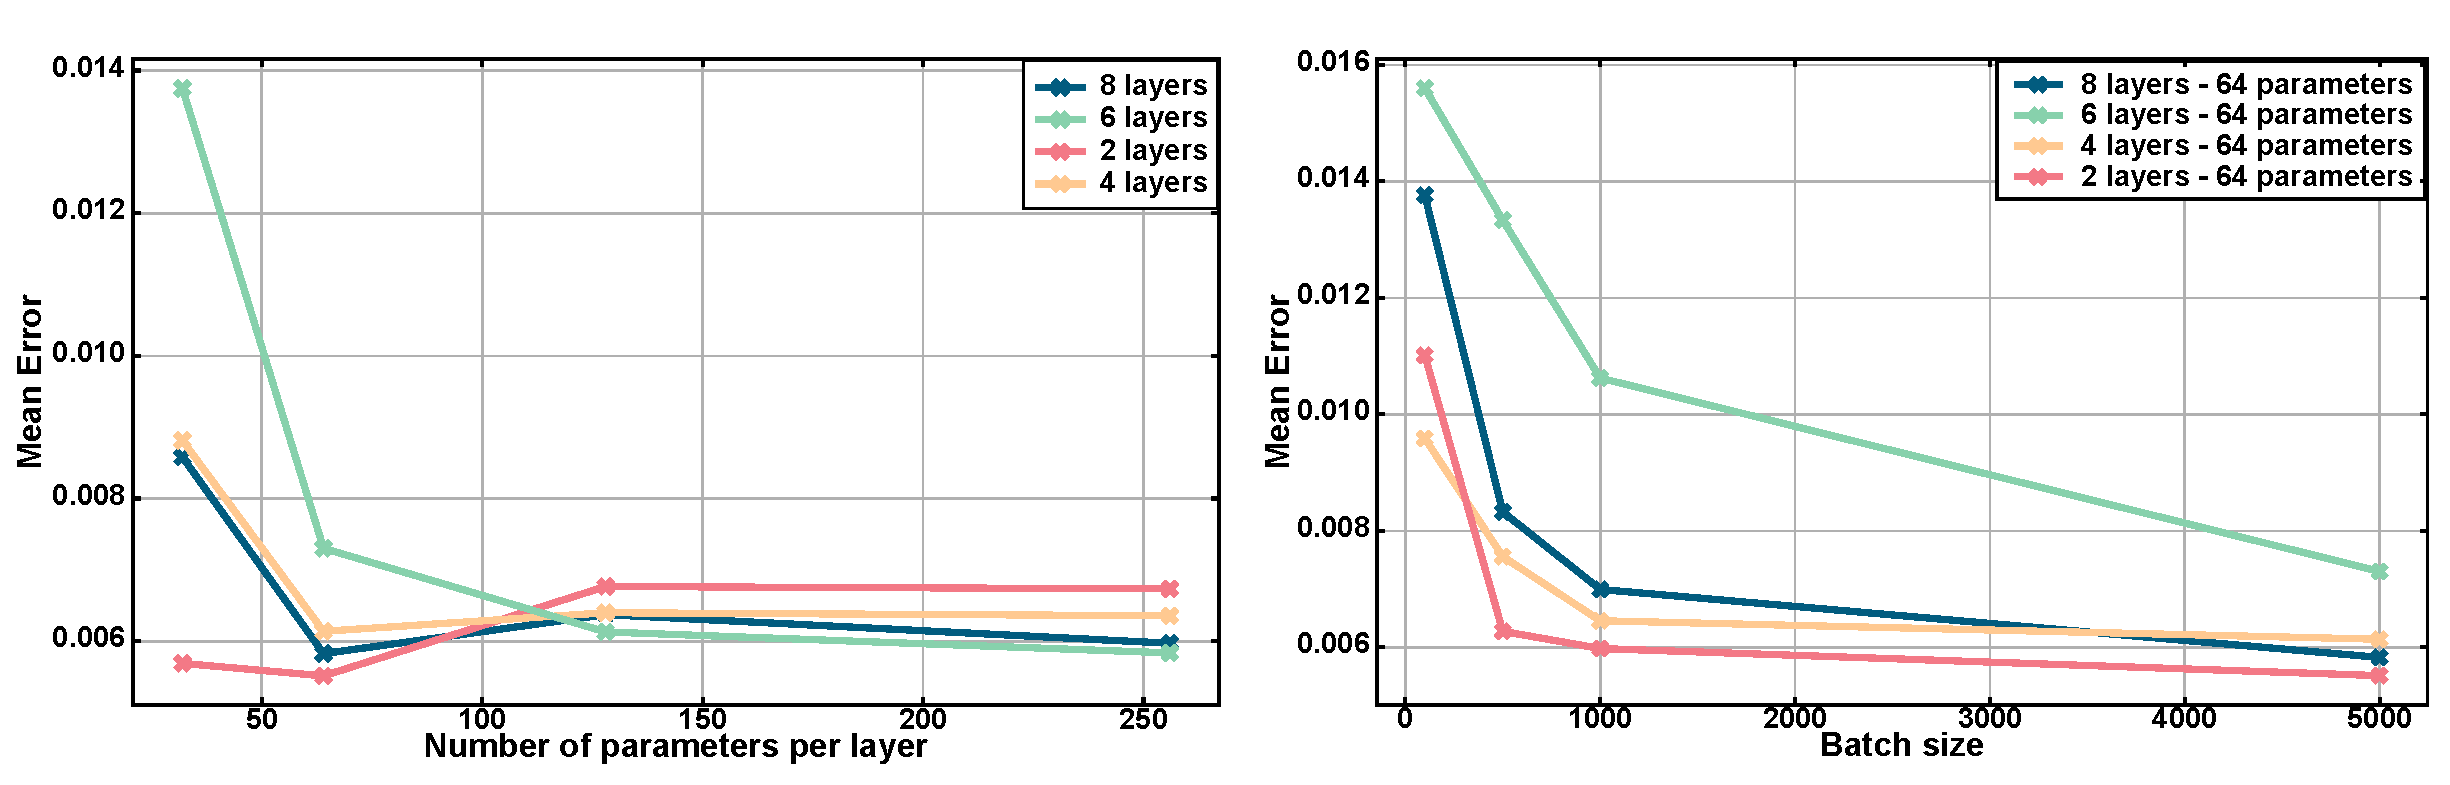
\includegraphics[width=\textwidth]{Figures/pot_combined2.pdf}
    
    \caption{We show results for different parameter settings using $\phi_n$ computed by the NeatSDF method as input geometry. \textbf{Left:} Mean error and number of parameters per hidden layer for varying number of layers and constant batch size, $bs = 5000$. 
     \textbf{Right:} Mean error and batch size for varying number of layers and fixed number of parameters. Both plots show only minor improvements for larger networks and batch sizes. For all following examples within this chapter, we choose 4 layers and 256 weights as our standard architecture, along with 5000 samples per batch.}
    \label{poisson_diff_bs}
    \end{figure}
 
At this point, we want to briefly outline the possibility of imposing boundary conditions for neural PDEs. Assume that we want to solve a PDE of the form $\mathbb{L}(u) = 0,$ with $  u:\Omega\subset\R^3\rightarrow\R$, for some differential operator $\mathbb{L}$ and Dirichlet boundary conditions $ u = g \text{ on }\partial\Omega$. One option is to impose the boundary condition variationally using an additional term in the loss functional: $$\mathcal L_{total}(u) = \mathcal{L}_{PDE}(u) + \lambda \int_{\partial \Omega} (u - g) ^2\, \mathrm{da}, \quad \lambda \in\R^+.$$
While straightforward to implement, this approach is undesirable for two main reasons: first, the boundary conditions are satisfied only approximately. These errors can propagate and influence the interior solution.  Second, the stability of the optimization process might be sensitive to the choice of the parameter $\lambda$.\par
In some cases, it is possible to impose boundary conditions \emph{exactly} within neural networks, as proposed by \cite{BERRONE2023e18820}. Let $\mathcal{N}_\theta: \R^3 \rightarrow \R$ denote an artificial neural network. To enforce the boundary conditions, we add one additional layer to the network architecture, which, for some input point $x_{in} \in \Omega$, multiplies the output $x= \mathcal N _\theta(x_{in})$  by a distance-like function $\psi: \R^3 \rightarrow\R$, resulting in 
\begin{align*}
    x_{out} &= \mathcal N_\theta(x_{in})\,\psi(x_{in}) + \hat g(x_{in}) \\&= x\,\psi(x_{in})+ \hat g(x_{in}).
\end{align*}
Here, $\hat{g}: \Omega \rightarrow\R$ denotes an extension of the boundary condition $g: \partial \Omega \rightarrow \R $ to the full domain $\Omega$: $\hat g|_{\partial \Omega} = g$. By "distance-like", we mean that $\psi(x) = 0 $ if and only if $ x \in \partial  \Omega$ and $\psi > 0$ in $\Omega$. Other kinds of boundary conditions, like Neumann and Robin, can be implemented using similar strategies. \par
For simple geometries of $\Omega$, for example, for polygonal domains, a polynomial distance-like function $\psi$ can be easily constructed analytically. For more complex geometries, one may instead employ a simple adaptation of the method described in \cref{SectionNeuralImplicitSurf}, to generate an \emph{unsigned} distance function with zero-level set $\mathcal M_0 = \partial \Omega$. We show quantitative results of this approach in \cref{poissonpb}.

\begin{figure}[t]
    \centering
    \begin{minipage}[c]{0.45\linewidth}
        \centering
        \begin{tabular}{lcc}
            \toprule
            \textbf{Method} &$\mathbf{\psi}$&\textbf{Mean error} \\
            \midrule
            HeatSDF &$1$     & 0.00589 \\
            HeatSDF & $|x_1|$     &  0.00715 \\
            NeatSDF& $ 1$     & 0.00583   \\
            NeatSDF& $|x_1|$     & 0.00421   \\
            \bottomrule
        \end{tabular}    
        
    \end{minipage}%
    \hspace{0.5em}
    \begin{minipage}[c]{0.4\linewidth}
        \centering
        \includegraphics[width=\linewidth]{Figures/potato.pdf}
    \end{minipage}
    \caption{We show the zero-level set of the input geometry (\textbf{top right}; side view) and the ground truth PDE solution (\textbf{bottom right}; top view). On the \textbf{left}, we present a quantitative error evaluation for both HeatSDF and NeatSDF based geometries, comparing boundary conditions fixed during ($|\psi|= x_1$ and $\hat g = 0$) versus after training ($|\psi| = 1$, $\hat g = 0$ and shift solution after training). The mean error is largely unaffected by the choice of how the boundary conditions are fixed.}
    \label{poissonpb}
\end{figure}

\subsection{Heat flow}\label{section_heatflow}
Next, we aim to solve the geometric heat equation, given by
\begin{align}\label{eq:heatflow}
    0 &= \partial_t w - \Delta_{\mathcal{M}_c} w,\notag \\
    w(0,\cdot) &= w^0 \in L^2(\mathcal{M}_c).  
\end{align}
Once again, the problem is well-defined without boundary conditions in space, since $\mathcal{M}_c$ is assumed to be closed.\\
We reformulate the PDE as a time-discrete variational problem:
\begin{align}\label{geometric_heat_eq}
    w^{1} \coloneqq \argmin_{w\in H^1(D)}\int_D (w - w^0)^2 + \tau \|\nabla_{\mathcal{M}}w\|^2 \,\mathrm{d}x
\end{align} for $\tau > 0 $, and solve in time, by iteratively using the solution from the previous step as initial data. Then $w^k$ denotes the approximation of the PDE solution at time $k\tau$, i.e., $w^k(\,\cdot\,) \approx w(k\,\tau, \,\cdot\,)$. Note that \cref{geometric_heat_eq} follows from \cref{eq:heatflow}, by approximating the time derivative via the implicit Euler scheme:  $$\partial_t w(k\tau, x) \approx \frac{w((k+1)\tau, x) - w(k\tau, x)}{\tau}. $$
First, we present experiments for initial data with $|\{w^0 \neq0\}| >0$, see \cref{comp_beethoven}. Here, $|\cdot|$ denotes the surface Lebesque measure, i.e., $$|\{w^0 \neq0\}| = \int_\mathcal{S} \chi_{\{w^0 \neq 0\}} \,\mathrm{da}\, {>} 0.$$
\begin{figure}
    \centering    
    \includegraphics[width = \textwidth, trim=2pt 2pt 2pt 2pt, clip]{Figures/Heatflow.pdf}
\caption{Visualization of two approximations of the heat flow for $|\{w^0 \neq0\}| >0$. We compare a FEM approximation on the ground truth mesh (\textbf{bottom}) with a neural narrow-band approximation using a signed distance function computed using the NeatSDF method as input geometry (\textbf{top}). The neural heat flow on the neural surface is qualitatively similar to the FEM solution.}\label{comp_beethoven}
\end{figure}

\begin{figure}
    
    \includegraphics[width = \textwidth, page =2 ]{Figures/bunnys_heatflow.pdf}
    
\caption{The figure shows a neural approximation of the heat equation for point initial data by first approximating the point source with a Gaussian of small variance (denoted as t = 0) and then using a locally refined box-grid ($k=3$) to iteratively approximate the subsequent time steps.} \label{point_bunny}
\end{figure}
For cases with lower-dimensional initial data, i.e. $|\{w^0 \neq0\}| = 0$, we propose the following strategy:
Assume for simplicity, that $w^0 = \delta_{x_0}$ for some $x_0\in\S$, then $|\{w^0 \neq0\}| = |\{x_0\}| = 0$. General lower-dimensional initial data can be handled in a similar fashion. To approximate the point source, we replace the Dirac delta with a smooth Gaussian function. Specifically, we define the regularized initial data as
\[
w^{\delta}(x) \coloneqq \alpha \sqrt{4\pi\delta} \, \exp\Bigg({-\frac{\|x - x_0\|^2}{2\delta}}\Bigg), \quad \alpha \in \mathbb{R}^+, \quad 0 < \delta \ll 1.
\]
This construction is motivated by the fundamental solution of the heat equation in \( \mathbb{R}^n \) (see, for example, \cite{evans2}), which is given by
\[
\Phi(t, x) = \frac{1}{(4\pi t)^{n/2}} \exp\Big({-\frac{\|x\|^2}{4t}}\Big).
\]
As \( t \to 0 \), this kernel converges in the sense of distributions to the Dirac delta. Thus, using a Gaussian of the form above with a small variance \( \delta \) provides a smooth approximation of a point heat source. This allows us to avoid the singularities associated with delta functions while still locally mimicking their influence.\par
In practice, we want to make $\delta$ as small as possible. However, taking $\delta$ small comes with increased demands on the sampling strategy, since we want to make sure that the region with $w^\delta >> 0$ is represented within each batch. To overcome this issue, we use an adaptive version of the box-algorithm presented in \cref{box_algorithm}: 
\begin{algorithm}\textbf{(Local Box-Grid Refinement:)}
\begin{enumerate}
    \item Extract a uniform box grid in the occupied region, as described in \cref{box_algorithm,clever_sampling}.
    
    \item Identify the box containing the point \(x_0\) and mark it as level \(k\), for a given \(k \in \mathbb{N}, k > 0\).
    
    \item Repeat the following process \((k - 1)\) times: for each box currently marked at level \(m \leq k\), mark all of its unmarked direct neighbors as level \(m - 1\).
    
    \item Subdivide each box based on its assigned level and store the corresponding box midpoints:
    \begin{itemize}
        \item Boxes at level \(k\) are subdivided \(k\) times,
        %\item Boxes at level \(k - 1\) are subdivided \(k - 1\) times,
        \item $\dots$
        \item Boxes at level \(1\) are subdivided once,
        \item Boxes at level \(0\) are not subdivided.
    \end{itemize}
    
    \item Apply the sampling strategy described in \cref{clever_sampling} to the midpoints of the refined boxes. This results in a higher sampling density near the initial point \(x_0\), which gradually decreases in regions farther away.
\end{enumerate}
\end{algorithm}
For our experiments, we divide one box into 27 smaller boxes for each level of subdivision, thus dividing the box edge length by three at each level.\\
Since the midpoints of the resulting grid now aren't uniformly distributed in $D$, we need to introduce integration weights to numerically evaluate the integrals: 
\begin{equation*}
    \min_{w\in H^1(D)} \frac{1}{N_{bs}} \sum_i^{N_{bs}} \omega_i \eta(\phi(x_i)) \left((w(x_i) - w^k(x_i))^2 + \tau \|\nabla_{\mathcal{M}(x_i)} w(x_i)\|^2\right).
\end{equation*}
In our case, $\omega_i\coloneqq (\frac{1}{27})^m$, for $x_i$ being sampled from the $i$-th box, which has been marked as level $m\leq k$. A qualitative result is shown in \cref{point_bunny}.
\begin{remark}\textbf{(Conservation:)}
    The weak formulation of the heat equation is \[
        \int_\mathcal{S} \partial_t u \, \psi + \nabla_\mathcal{S} u \cdot \nabla_\mathcal{S} \psi \, \mathrm{da} = 0, \quad \forall \psi\,\in \mathcal C^\infty(\S).
    \]
    Taking $\psi = 1$ yields the conservation equation
    $$\frac{d}{dt} \int_\S  u \,\mathrm{da} = 0,$$
    thus, the overall "heat mass" is conserved over time.
\end{remark}
 We show that the neural narrow-band method is able to approximately conserve the heat mass over time, see \cref{mass_conservation}.
 \begin{figure}[htbp]
  \centering
  \begin{minipage}[l]{0.7\textwidth}
    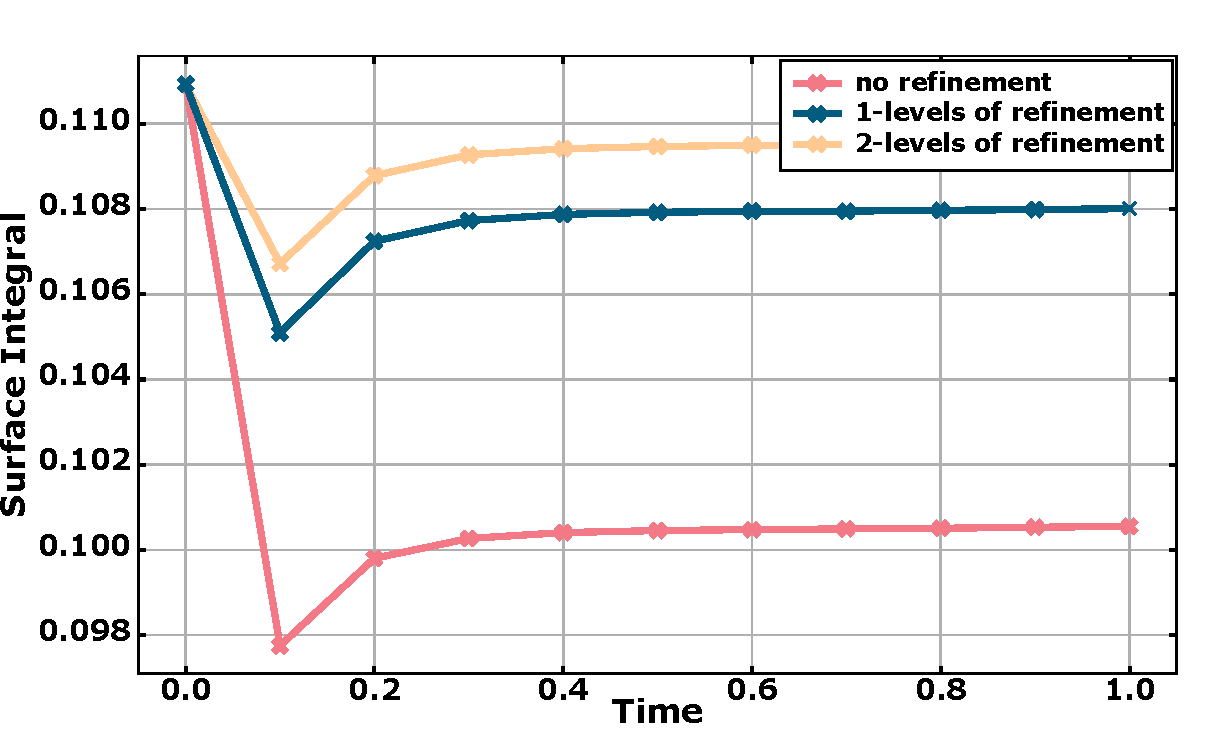
\includegraphics[width=\linewidth]{Figures/heatflow_conservation}
  \end{minipage}%
  \hfill
  \begin{minipage}[r]{0.29\textwidth}
    \captionof{figure}{Our method approximately conserves total heat over time and shows improved accuracy with increased sampling density near the point source. For these experiments, we used the geometry and initial data shown in \cref{point_bunny}.}
    \label{mass_conservation}
  \end{minipage}
\end{figure}
\FloatBarrier
\subsection{Geodesics in Heat}
We proceed by adapting the heat method, to compute geodesic distances on a neural surface; the heat method was originally developed in the discrete setting by \cite{Crane_2013}, To this end, we solve the heat flow as described in \cref{section_heatflow} and then normalize the resulting vector field to obtain distance estimates on the zero-level set. For more details regarding the heat method, see the discussion in \cref{SDF_rel_work}. \newpage
To this end, we solve two problems, namely we
\begin{enumerate}
    \item solve the heat equation $\partial_t u - \Delta_{\mathcal{M}_c} u = 0$ for some fixed time $\tau$ and given initial data $u_0$, and then
    \item solve the Poisson problem $\Delta_{\mathcal{M}_c} w = \operatorname{div}_{\mathcal{M}_c}  n$, for $ n = -\frac{\nabla_{\mathcal{M}_c} u}{\|\nabla_{\mathcal{M}_c} u\|}$.
\end{enumerate}
Overall, this approach is conceptually similar to the SDF framework, which we introduced in \cref{section_SDFmethod}. 
It is worth noting that we now calculate distances on $\S$ instead of $\R^n$; furthermore, we are only interested in \emph{unsigned} distance functions. This significantly simplifies the computation.\par
We solve both steps using the neural narrow-band method presented above (see \cref{section_heatflow,section_PoissonPB}), with one minor change: the variational Poisson problem in the heat method (step (ii)) reads
$$\min_{w\in H^1(D)}\int_D \frac{1}{2}\|\nabla_\mathcal{M}w\|^2 + \nabla_{\mathcal{M}} \cdot n \, w \,\mathrm{d}x, \quad \text{where } n = - \frac{\nabla_{\mathcal{M}} u}{\|\nabla u_{\mathcal{M}}\|},$$
thus requiring second derivatives of the heat solution $u$. Experiments show that our approximations of $u$ are not smooth enough to compute consistent second derivatives. We can overcome this issue here by integrating the force term by parts. Then the problem reads 
$$\min_{w\in H^1(D)}\int_D \frac{1}{2}\|\nabla_\mathcal{M}w\|^2 - n\cdot \nabla w \,\mathrm{d}x.$$
\paragraph{Implementation details:}
For the Poisson problem, step (ii), we need to introduce boundary conditions; more precisely, we want to impose zero boundary values at the initial heat source, $w(x) = 0$ if $u_0(x) \neq 0 $. As above, we solve the problem without boundary conditions and afterwards shift the solution, $w = w_{neural} - w_{neural}(x_0).$\par
We computed geodesic distances using several time steps, and found that \( t \in [0.3, 0.5] \) (depending on the overall size of the object) yields the best balance between precision near the source point and accuracy farther away.

\begin{figure}[htbp]
  \centering
  \begin{minipage}[c]{0.45\textwidth}
    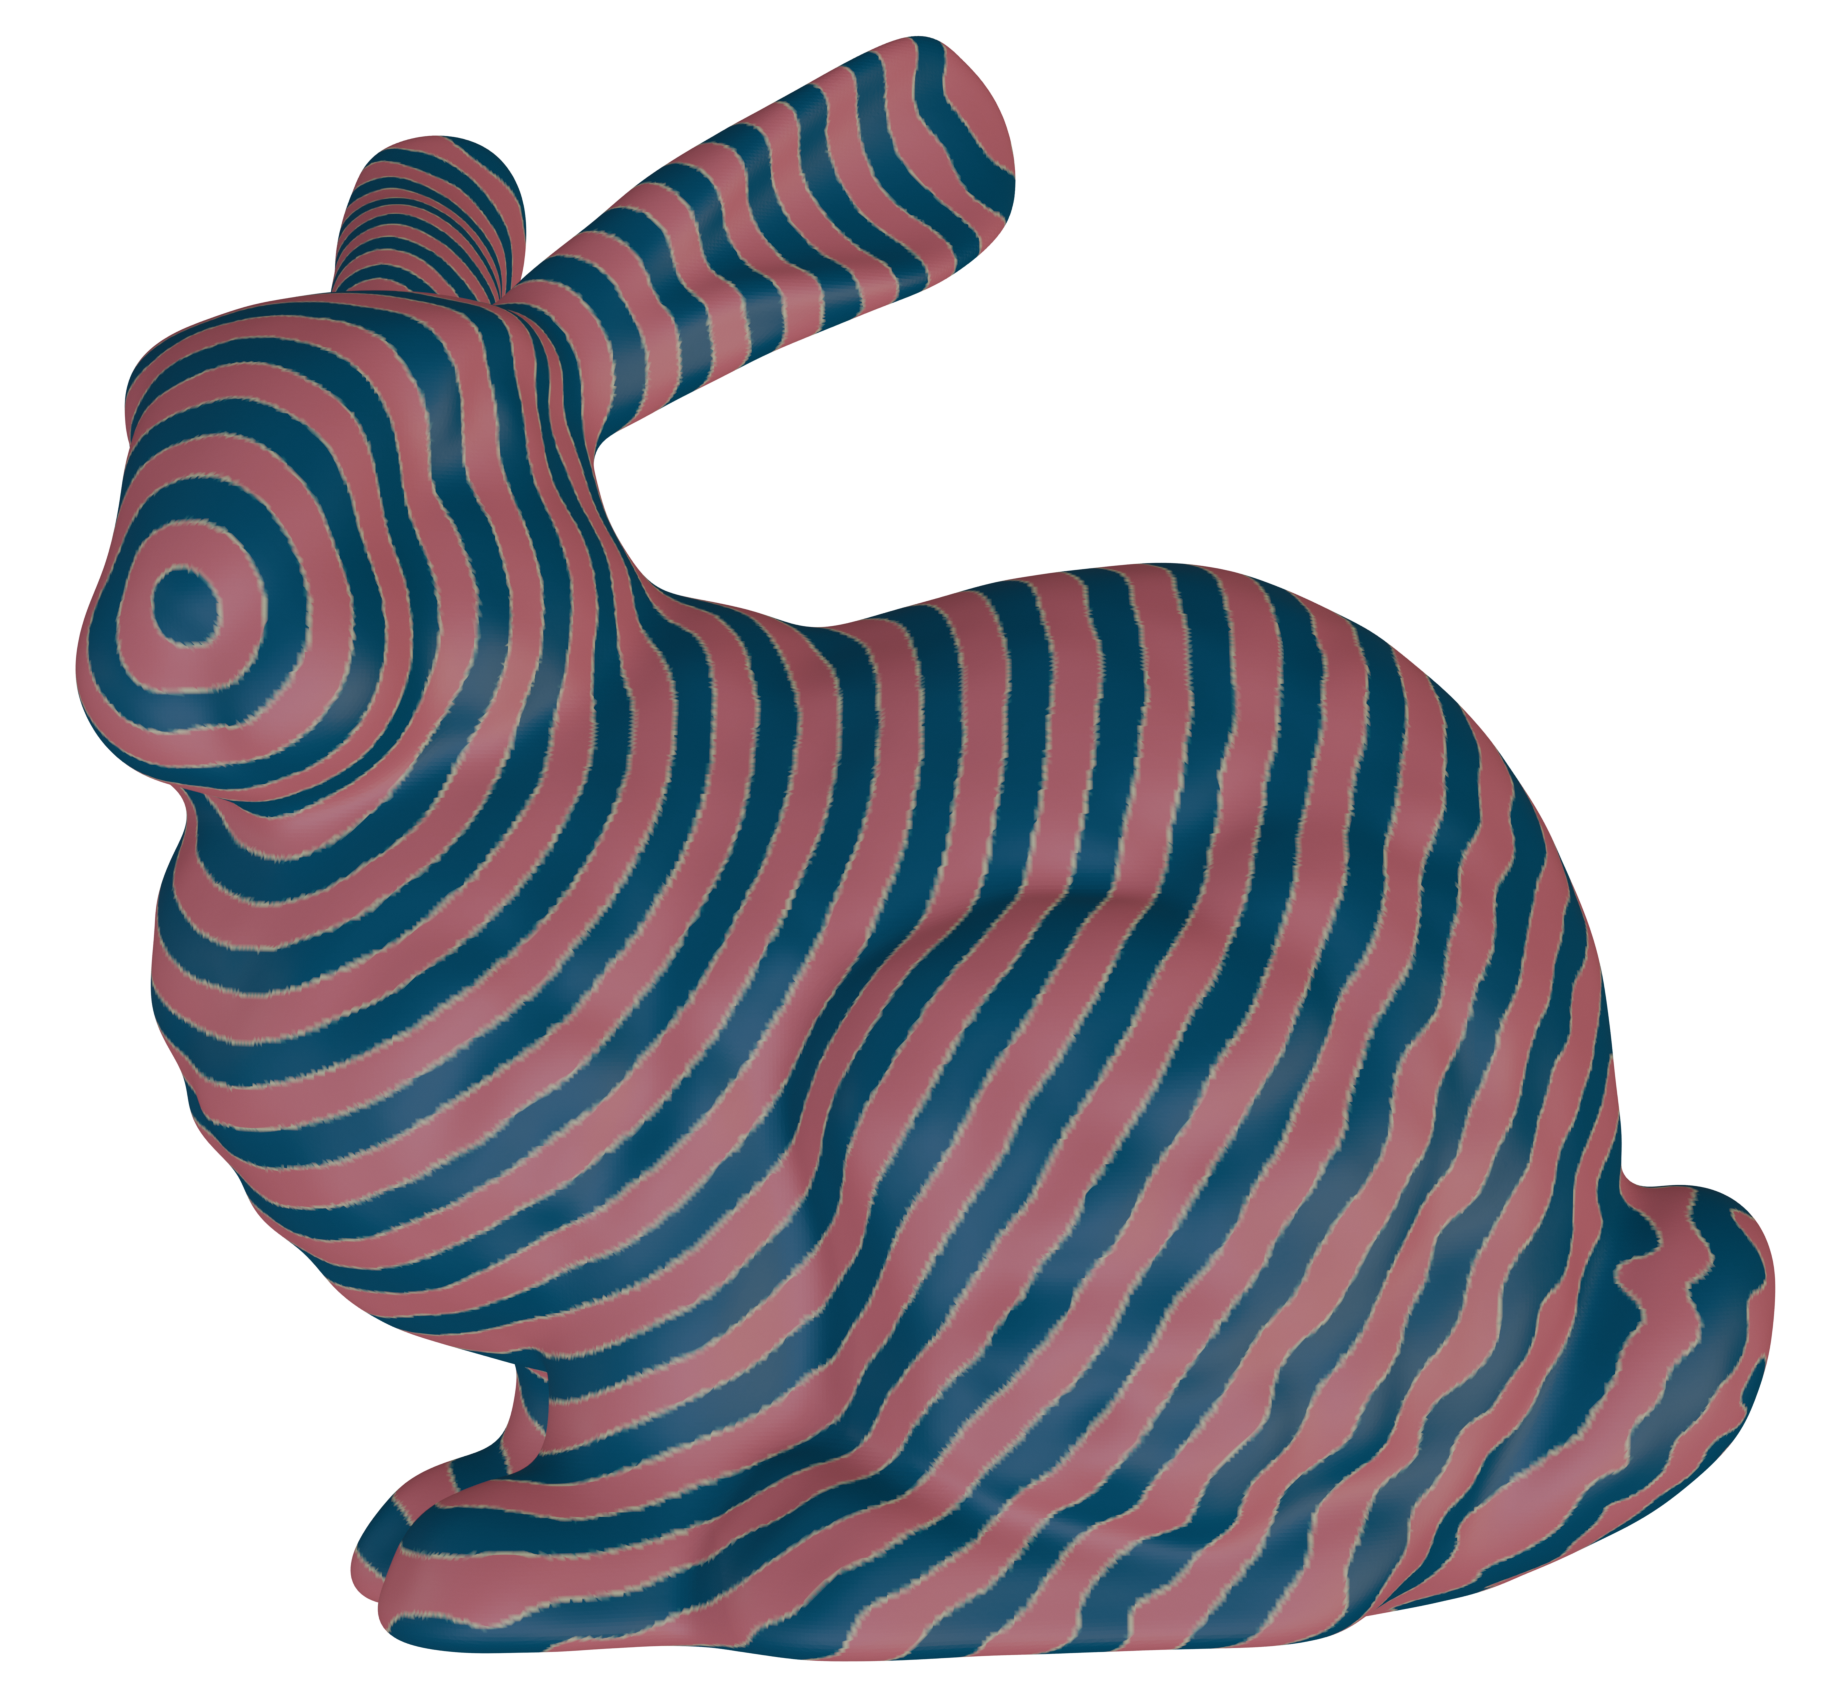
\includegraphics[width=\linewidth]{Figures/geodesics_striped.png}
  \end{minipage}%
  \hfill
  \begin{minipage}[c]{0.45\textwidth}
    \captionof{figure}{For the same initial data as in \cref{point_bunny} and with a maximal refinement level of $k=3$, we compute geodesic distances using the neural heat method. For the heat flow, we used one time step of size $\tau = 0.3$. For visualization, we color the mesh according to the approximated function values with equidistant color stripes of width $0.05$.}
    \label{fig:geodINHeat2}
  \end{minipage}
\end{figure}

\begin{figure}
    \includegraphics[width = \linewidth]{Figures/geodesics_spiral.pdf}
\caption{Starting from an approximated point source (\textbf{left}), we first solve the heat equation for a larger time step, $\tau = 0.5$ (\textbf{middle}). Based on this result, we compute geodesic distances on the surface using the neural heat method (\textbf{right}). For visualization, the mesh is color-coded according to the approximated function values, using equidistant color bands of width $0.05$ (\textbf{bottom right}) and equidistant isolines (\textbf{top right} and \textbf{middle}). The approximated distances for regions farther away from the point source become unreliable (see \textbf{right}, regions near the endpoint of the spiral).}\label{}
\end{figure}

\clearpage
\chapter{Conclusion}
\begingroup
\let\clearpage\relax
\section{Limitations}
\paragraph{Neural SDFs:} Despite the effectiveness of the proposed methods, several limitations remain. For the SDF approach, one key issue is the reliance on the box algorithm to distinguish between the inside and outside regions of the geometry. As discussed earlier, this algorithm may fail in certain cases. While we proposed to compute generalized winding numbers as a more robust alternative, this approach requires significantly more precomputation. Another limitation of our SDF methods is the training of two separate neural networks; this increases the complexity of the training pipeline and may also extend the required computation time. Furthermore, we point out that the NeatSDF method requires more time to compute per iteration than the HeatSDF method, since we additionally need to compute second derivatives.
\paragraph{Neural PDEs:} The neural narrow-band method also faces certain challenges. Accurately computing second-order derivatives through the neural network is difficult, limiting the method's applicability to problems involving higher-order differential operators, such as surface evolution via mean curvature flow. Furthermore, enforcing most boundary conditions post-training restricts the method's generality. Currently, there are no general and easy-to-use ways to impose boundary conditions. 
\section{Outlook and Future Work}
Neural orientation methods reduce the need to compute signed distance functions from \emph{unoriented} point clouds. In scenarios where normal information is available or can be reliably estimated, we propose incorporating an on-surface normal loss, which could enhance the model's accuracy, potentially in combination with loss terms from HeatSDF or NeatSDF. Preliminary experiments suggest that such a loss function can recover SDFs without requiring explicit inside/outside segmentation, thereby reducing the need for extensive preprocessing.\par
Additionally, a neural adaptation of the method proposed by \cite{FengCrane} offers a promising direction for defining yet another head-based neural SDF approach. As a first step, we would diffuse the normals of an oriented point cloud, yielding a continuous normal field. This field could be used in a manner similar to our heat step.\par
We also aim to improve the proposed narrow-band framework to make it usable for higher-order partial differential equations. In particular, we are interested in exploring the potential of neural networks for modeling surface deformations.\par
Beyond these topics, some more general questions remain. For example, the use of more advanced network architectures, such as ResNet (\cite{he2015deepresiduallearningimage}) appears promising for improving approximation quality. \par
Additionally, it remains unclear whether an experimental convergence behavior can be established for the proposed methods.
\endgroup
{
%\footnotesize
\setlength{\bibsep}{7pt}
\bibliographystyle{plainnat}
\bibliography{references.bib}
}

\appendix
\chapter{Theoretical Background}\label{appendix:A}
The following appendix contains supplementary proofs and theoretical results used but not proven in the main text.
\begin{proof}[Proof of \cref{technicalLemma}]
    Let $\phi_i\in H^1(\Omega)$, such that $\phi_i\xrightharpoonup{H^1(\Omega)} \phi$, and let $n\in L^2(\Omega, \R^3)$ be approximated by a sequence of smooth and compactly supported functions \mbox{$(n_k)_{k\in \mathbb N}\subset C_c^\infty(\Omega, \R^3)$}, with $n_k \xrightarrow{L^2(\Omega)} n$. Then $ \forall k\in \mathbb N, \, \forall \phi \in H^1(\Omega):$
    $$\int_\Omega \nabla |\phi|\cdot n_k \,\mathrm{d}x = - \int_\Omega |\phi| \nabla \cdot n_k \,\mathrm{d}x,$$
    where we used integration by parts. Thus, the map $$
    H^1(\Omega) \rightarrow\R,\quad
        \psi \mapsto \int_\Omega \nabla |\psi|\cdot n_k \,\mathrm{d}x,
     $$ 
    is $L^2$-continuous for fixed $k\in \mathbb N$. By Rellich's theorem $$\lim_{i\rightarrow\infty}\int_\Omega \nabla |\phi_i|\cdot n_k \,\mathrm{d}x = \int_\Omega \nabla |\phi|\cdot n_k \,\mathrm{d}x, \quad \forall k.$$ Further, we have
    \begin{align*}
        &\left|\int_\Omega \nabla |\phi_i|\cdot n \,\mathrm{d}x - \int_\Omega \nabla |\phi|\cdot n \,\mathrm{d}x\,\right|\\\displaybreak[3]
       \overset{\Delta\text{-ineq.        }\,}{\leq} &\left|\int_\Omega \nabla |\phi_i|\cdot n_k \,\mathrm{d}x - \int_\Omega \nabla |\phi|\cdot n_k \,\mathrm{d}x\,\right| \\&\quad \quad + \left| \int_\Omega \nabla |\phi_i| \cdot (n_k - n) \, \,\mathrm{d}x\, \right| 
 + \left| \int_\Omega \nabla |\phi| \cdot (n_k - n) \, \,\mathrm{d}x\, \right|\\
       \overset{\text{Hölder}}{\leq} &\left|\int_\Omega \nabla |\phi_i|\cdot n_k \,\mathrm{d}x - \int_\Omega \nabla |\phi|\cdot n_k \,\mathrm{d}x\,\right| \\  &\quad \quad+ \|\nabla \phi_i\|_{L^2(\Omega)} \|n_k - n\|_{L^2(\Omega)}  + \|\nabla \phi\|_{L^2(\Omega)} \|n_k - n\|_{L^2(\Omega)}\\ 
       \overset{\phi, \phi_i \in H^1 }{\leq} &\left|\int_\Omega \nabla |\phi_i|\cdot n_k \,\mathrm{d}x - \int_\Omega \nabla |\phi|\cdot n_k \,\mathrm{d}x\,\right| + C\|n_k - n\|_{L^2(\Omega)},
    \end{align*}
    for some constant $C\in \R^+$.    Therefore, we have that for all $k$ $$\limsup_{i\rightarrow\infty} \,\left| \int_\Omega \nabla |\phi_i|\cdot n \,\mathrm{d}x - \int_\Omega \nabla |\phi|\cdot n \,\mathrm{d}x\,\right| \leq C\|n_k - n\|_{L^2(\Omega)},$$ and taking $k\rightarrow\infty$ we conclude $$\int_\Omega \nabla |\phi_i|\cdot n \,\mathrm{d}x \rightarrow\int_\Omega \nabla |\phi|\cdot n \,\mathrm{d}x.$$
\end{proof}
\begin{theorem}\label{min_lsc}
    Let $u:\R^3\rightarrow\R$ and $n: \R^3\rightarrow\R^3$ . For any $\epsilon \in \R^+$, we have that $$G(\nabla u) \coloneqq \int_\Omega \min (\epsilon; \|\nabla u+ n\|^2,\|\nabla u - n\|^2)\,\mathrm{d}x$$ is lower semicontinuous with respect to weak $L^2$-convergence. Additionally, after adding the loss terms $\mathcal{E}_{surf}$ and $\mathcal{E}_{bd}$, the loss functional is coercive.\\
    Here $\min(\epsilon;a,b) \coloneqq \frac{a + b}{2} - \frac{1}{2}\sqrt{(a-b)^2 + \epsilon}$, for $\,a,\,b \in \R$ and obviously for $\epsilon  \rightarrow 0$ we have $\min(\epsilon; \cdot, \cdot) \rightarrow \min(\cdot, \cdot)$. 
\end{theorem}
\begin{proof}
\textbf{Weak lower semicontinuity:} We first notice that, just like in \cref{ProofExSDF}, we have that $$\|\nabla u \pm n\|^2 = \|\nabla u\|^2 \pm 2 \nabla u \cdot n + 1.$$
    We can thus rewrite $$\sqrt{(\|\nabla u + n\|^2 - \|\nabla u - n\|^2)^2 + \epsilon} = \sqrt{(4 \nabla u\cdot n)^2 + \epsilon}$$
    Overall we have \begin{align*}
        \min (\epsilon; \|\nabla u+ n\|^2,\|\nabla u - n\|^2) = \|\nabla u\|^2 + 1 + \sqrt{(4 \nabla u\cdot n)^2 + \epsilon}=: F(\nabla u). 
    \end{align*}
    Since $v\mapsto\sqrt{(4 \nabla u\cdot n)^2 + \epsilon}$ is convex as the composition of a convex function with a convex quadratic, and furthermore the sum of convex functions is convex, we conclude  that $F :\R^3 \rightarrow\R$ is convex. Thus, $\int_\Omega F(\nabla u)\, \mathrm{d}x$ is weakly lower semicontinuous, see \cref{thm:Tonelli}.\\
    \textbf{Coercivity:} Analog to the work done in \cref{ProofExSDF} we can estimate $$\|\nabla u\|^2_{L^2(\Omega)} \leq 2 \int_\Omega \|\nabla \phi \pm n\|^2 + \|n\|^2\,\mathrm{d}x.$$
    We claim that $\min_\epsilon(\cdot, \cdot) + C(\epsilon) \geq \min(\cdot, \cdot)$, for some $C(\epsilon) > 0$. If the claim is true, then ultimately 
    \begin{align*}
    \lambda_2\|\nabla \phi\| ^2_{L^2(\Omega)} + \lambda_1 \|\phi\| ^2_{L^2(\S)}
 &\leq 2 \lambda_2\int_\Omega\min_\epsilon(\|\nabla \phi + n\|^2, \|\nabla \phi - n\|^2) \,\mathrm{d}x \\ 
 &+ \lambda_1 \|\phi\| ^2_{L^2(\S)} + \lambda_3 \mathcal{E}_{bd} + C(\epsilon),
\end{align*} 
and with the same arguments as in \cref{ProofExSDF}, we conclude that the NeatSDF loss functional is coercive.\\
To show that indeed $\min_\epsilon(\cdot, \cdot) + C(\epsilon) \geq \min(\cdot, \cdot)$, we first rewrite $\min(a,b) = \frac{a+b}{2} - \frac{|a-b|}{2}$. The first term $\big(\frac{a+b}{2}\big)$ appears in both $\min_\epsilon$ and $\min$. Let $x \coloneqq |a-b|$, then we need to show, that $\sqrt{x^2 + \epsilon } -x \leq C(\epsilon) \coloneqq \sqrt{\epsilon}$. This estimate shows that \(\min_\epsilon(a, b)\) is uniformly bounded from below by \(\min(a, b)\) up to an error of \(\sqrt{\epsilon}\), 
which ensures that the regularized minimum remains coercive in the limit \(\epsilon \to 0\). \\
Indeed: $$\sqrt{x^2 + \epsilon } -x = \frac{(x^2+\epsilon) - x^2}{\sqrt{x^2+\epsilon} + x} = 
\begin{cases}
= \sqrt{\epsilon} & \text{if } x = 0 \\
< \sqrt{\epsilon} & \text{if } x > 0
\end{cases}$$

This ends the proof.
\end{proof}
\clearpage
\chapter{Additional Experimental Details}\label{appendix:B}
All code developed for this thesis is publicly available in the following GitHub repository: 
\href{https://github.com/sweidemaier/NeatSDF}{NeatSDF} 
(\url{https://github.com/sweidemaier/NeatSDF}).
\begin{table}
    \begin{tabular}{p{3.3cm} p{7cm} p{2.2cm}}
    \toprule
    \textbf{model} &\textbf{source}& \textbf{cloud size} \\
    \midrule
    Armadillo &\cite{DBLP:conf/siggraph/KrishnamurthyL96} & 170k \\
    Beethoven& \cite{threedscans}&390k \\
    Bird & \cite{Thingi10k}  (id 178340)& 100k \\
    Bucky & \cite{Thingi10k} (id 41140)& 100k\\
    Bunny &\cite{DBLP:conf/siggraph/TurkL94} & 170k \\
    Dog &\cite{dyke2020shrec} & 100k \\
    Gargoyle&\cite{reconbenchmark}&100k\\
    Hand &\cite{yeh2010template} & 6k\\
    Headphones& \cite{giga-headphone}&10k\\
    Lightbulb & \cite{Thingi10k} (id 39084) & 500k\\
    Max Planck head &\cite{Ivri2002divide} & 200k \\
    Pipes&  \cite{Thingi10k} (id 53754) & 100k\\
    \bottomrule
\end{tabular}
    \caption{Considered models and approximate point cloud sizes used as training input. \label{tab:meshes}}
\end{table}
\begin{figure}
    \centering
    \includegraphics[width=0.8\textwidth]{Figures/HeatSDF_isosurfaces.pdf}
    \caption{Extracted hypersurfaces $\mathcal{M}_c$ at different values $c$ for SDFs constructed using the HeatSDF method.}
\end{figure}
\begin{figure}
    \centering
    \includegraphics[width=0.9\textwidth, page = 2]{Figures/NeatSDF_isosurfaces.pdf}
    \caption{Extracted hypersurfaces $\mathcal{M}_c$ at different values $c$ for SDFs constructed using the NeatSDF method.}
\end{figure}
%

\end{document}
 